\documentclass[11pt,letterpaper]{article}
%%%%%\usepackage{cite}
\usepackage{amsmath}
\usepackage{amsfonts}
\usepackage{array}
\usepackage{dsfont}
\usepackage{amssymb}
\usepackage{amsthm}
\usepackage{bbold}
\usepackage{fullpage}
\usepackage{mathtools}
\usepackage{enumitem}
\usepackage{mathrsfs}
\usepackage[margin=0.9 in,headsep=0.3 in]{geometry}
\usepackage{hyperref}
\usepackage{graphicx}
\usepackage{gensymb}
\usepackage{xcolor,colortbl}
\usepackage[format=plain,
labelfont={bf,it},
textfont={it}]{caption}
\usepackage{float}
\usepackage{multirow}

\usepackage[backend=biber, style=ieee]{biblatex}
\addbibresource{Bibliography.bib}

%%%%%%%%%%%NEW PACKAGES I'VE ADDED FOR THE PURPOSE OF THESIS
\usepackage{amsthm}
\theoremstyle{definition}
\newtheorem{defn}{Definition}[section] % definition numbers are dependent on theorem numbers

\usepackage{newclude}
\usepackage{tikz}
\usetikzlibrary{shapes.geometric, arrows}
%%Define the two block types and arrow type for our flow diagram
\tikzstyle{startstop} = [rectangle, rounded corners, minimum width=3cm, minimum height=1cm,text centered, draw=black, fill=white]
\tikzstyle{process} = [rectangle, minimum width=3cm, minimum height=1cm, text centered, draw=black, fill=white]
\tikzstyle{arrow} = [thick,->,>=stealth]
%%%%%%%%%%%END OF NEW PACKAGES I'VE ADDED FOR THE PURPOSE OF THESIS

\newcommand*{\SignatureAndDate}[1]{%
	\par\noindent\makebox[2.5in]{\hrulefill} \hfill\makebox[2.0in]{\hrulefill}%
	\par\noindent\makebox[2.5in][l]{#1}      \hfill\makebox[2.0in][l]{Date}%
}%
\newcolumntype{L}{>{\centering\arraybackslash}m{2cm}}
\newcolumntype{P}{>{\centering\arraybackslash}m{3cm}}
\newcolumntype{Q}{>{\centering\arraybackslash}m{4cm}}
\setlength{\parindent}{0em}

\allowdisplaybreaks

\newcommand{\R}{\mathds{R}}
\newcommand{\Z}{\mathds{Z}}
\newcommand{\Rplus}{\mathds{R}_{> 0}}
\newcommand{\Zplus}{\mathds{Z}_{\geq 0}}
\newcommand{\F}{\mathds{F}}
\newcommand{\N}{\mathds{N}}
\newcommand{\T}{\mathds{T}}
\newcommand{\s}{\mathds{S}}
\newcommand{\C}{\mathds{C}}
\newcommand{\CDFT}{\mathscr{F}_{CD}} %Fourier transform
\newcommand{\ip}[2]{\langle #1, #2\rangle}

\setlength{\parskip}{0.5em}

\usepackage{fancyhdr}
\setlength{\headheight}{15.2pt}
\pagestyle{fancy}
%%\fancyhead[RE]{\thepage}
%%\fancyhead[ER]{\rightmark}
\fancyhead[LE,RO]{\slshape \rightmark}
\fancyhead[LO,RE]{\slshape \leftmark}
\fancyfoot[C]{\thepage}

\makeatletter
\newsavebox\myboxA
\newsavebox\myboxB
\newlength\mylenA

\title{ A-1: Modelling and Control of a Ripstik\textsuperscript{\textregistered} \\MTHE 493 Final Report}
\date{Friday April $7^{\textrm{th}}$, 2017}
\author{\\Andrew Cantanna (10092489) \\Cameron Hudson (10092287)\\
	Benjamin Rudson (10083664)\\}
\begin{document}

	\begin{titlepage}
		\maketitle
		\thispagestyle{empty}		
	\end{titlepage}
	\newpage
	\pagenumbering{Roman} 
	%%\pagestyle{myheadings}
\begin{abstract}
	This is the abstract.
\end{abstract}	
\clearpage
\newpage
\begin{center}
\textbf{Acknowledgements}
\end{center}

\newpage	
	\renewcommand{\baselinestretch}{0.75}\normalsize
	\tableofcontents
	\renewcommand{\baselinestretch}{1.0}\normalsize

\newpage
\listoffigures
\newpage
\listoftables


\clearpage
\pagenumbering{arabic}
	
	\newpage



	\pagestyle{fancy}
\section{Introduction}
\subsection{Context \& Motivation}
%Introduce most of the concepts around money in electric transportation/urbanization/environmental aspects from the presentation, e.g. "why is this needed"
\subsection{Changing Cities}

By 2050, it is projected that 86 \% of the developed world will reside in urban areas \cite{Economist}. 
As a result of the adoption of the motorized vehicle, cities have become increasingly multi-centred, with retail parks and industrial estates far removed from the city centre \cite{SustainableTransport}. 
As a result of the changing layout of modern cities, traditional public transport has been rendered largely ineffective at efficiently transporting the population within the city \cite{SustainableTransport}. 
A British study showed that 83\% of commuting trips and 90\% of business trips in that country involved only a single passenger in a car \cite{NTS}, highlighting that the supply of mass, group transit does not meet the travel demands of modern society.
\\
\\
The lack of effective transportation infrastructure also has a considerable impact on the environment. 
The United States Environmental Protection Agency has determined that 14\% of global emissions are as a result of the transportation sector \cite{EPA}. 
Meanwhile, a Belgian case study showed that 47\% of trips and 54\% of distance travelled in that country was for the purpose of urban commuting \cite{Belgium}. 
Clearly, the environmental impact of urban transportation is considerable.

It has been determined that an effective transportation system for a modern city must satisfy the following constraints \cite{SustainableTransport}:

\begin{enumerate}
	\item is available on demand
	\item goes non-stop from start to destination
	\item is easily accessible and offers a full choice of destinations
	\item is strongly environmentally friendly
	\item is low cost
	\item integrates well with other forms of transport
	\item has demonstrably high safety together with personal security
\end{enumerate}

Personal electric transport (PET) has the potential to satisfy the transportation demands of a modern city. 
PET is user operated, meaning it is indeed available on demand and is accessible. 
Additionally, it is inherently portable and thus integrates well with other forms of transport. 
Using an appropriate power source will ensure that the PET device can travel non-stop to and from a multitude of destinations at a low cost. 
In order to ensure personal security and safety, it is imperative that the PET device have a stabilizing mechanism governed by control law. 
A RipStik makes for an ideal candidate in the study of control law for complex mechanical systems for use in personal electric transport. 


\subsubsection{The RipStik}

A caster board, known commercially as a RipStik, is a two-wheeled, human powered vehicle. 
The board is similar to a skateboard; however, it features two platforms, each with a wheel connected to an inclined free spinning caster. 
These platforms are connected by a torsion bar. 
This gives the caster board rider the unique ability to generate propulsion without removing their feet from the board through a series of small turns. 
This configuration also allows for tighter turning and more responsive speed control when compared to a skateboard. 

\begin{figure}[!htb]
	\centering
	\minipage{0.5\textwidth}
	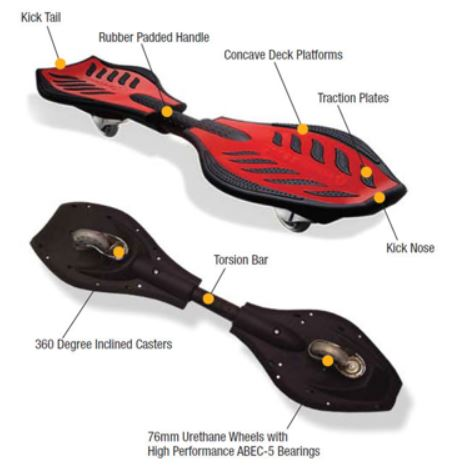
\includegraphics[width=\linewidth]{RipStik.JPG}
	\caption{Detailed description of the components of a RipStik \cite{PIC}}\label{fig:RipStik}
	\endminipage
\end{figure}
\par
The RipStik presents an interesting research opportunity because the associated motions and physics are unintuitive.
As a result, comprehensive testing and design metrics are required as there are no implicit assumptions to be made about the device's operation. 
This allows the technology developed in modelling and controlling the RipStik to be applied to a large variety of systems; furthermore, many of the core concepts like wheel motion and stability are highly applicable in the domain of electric transportation. 

The design of a control system for a personal transportation device needs to be done with careful consideration for a number of external factors. 
Aside from the challenges associated with the development of the mathematical model and control system, issues pertaining to the patents for transport systems \cite{casterboardPatent} and restricted operation of certain devices \cite{TOLaws} may represent a barrier in bringing theses products to market. 
Additionally, a mechanical system will be required to execute the commands of the control system. 
The difficulties associated with the recycling of batteries \cite{BatteryRecharge}, housing \cite{PlasticAssessment} and motors may threaten the environmental feasibility of the final design. 
The system may also be susceptible to "hacking" by outside sources \cite{DEFCON}, which could pose a significant safety risk to the operator. 
These issues will be analysed to mitigate the associated risks and properly weigh relevant environmental, social and economic tradeoffs.
This area of study has the potential to redefine urban commuting across the world by introducing a safe, cost-effective and environmentally-friendly option for short distance travel. 

\subsection{Problem Definition}

Aside from select innovative exceptions, current methods of electric personal transport are limited in both mechanics and utility by an adherence to more traditional form factors including the skateboard and bicycle. 
As an example of an alternate transportation system, a full control law for a RipStik will be developed and tested. 
The development of this control law will first require a complete, working mathematical model of the RipStik and a custom tool to visualize the model and control law outputs on a 3D model of the RipStik. 
Simplifications and assumptions will need to be made in order to develop a working model of the system. 
These simplifications and assumptions will be carefully scrutinized to ensure that they do not compromise the ability of the model to be applied to other complex mechanical systems. 
A control system will then be developed to propel the RipStik with consideration to triple bottom line implications, including minimizing power requirements and ensuring operator safety. 
Tradeoffs will be made in the development of the control system to find the optimal system which satisfies the performance constraints of the problem and optimizes triple bottom line impact. 

\subsection{Technical Background}
A number of mathematical tools were utilized to develop the framework necessary for the mathematical modelling and control of the RipStik.

\subsubsection{Euler Angles}

Euler angles were introduced to describe the orientation of a body in an inertial reference frame.
These orientations were represented by rotations of three angles; yaw ($\theta$), pitch ($\psi$), and roll ($\alpha$).
With the Euler angles defined, rotation matrices can then be created for the bodies of a system.

A rotation matrix can be defined in the following way \cite{Lewis}:

\begin{equation}
\label{eq:RotM}
R =
\begin{bmatrix} 
\cos\alpha\cos\psi & \cos\alpha\sin\psi\sin\theta - \cos\theta\sin\alpha &\cos\alpha\cos\theta\sin\psi+\sin\alpha\sin\theta\\
\cos\psi\sin\alpha & \cos\alpha\cos\theta+\sin\alpha\sin\psi\sin\theta & \cos\theta\sin\alpha\sin\psi - \cos\alpha\sin\theta\\
-\sin\psi & \cos\psi\sin\theta & \cos\psi\cos\theta 
\end{bmatrix}
\end{equation}

The rotation matrix R can be used to describe a rotation from a body-fixed frame to the inertial frame \cite{VTOL}.

\subsubsection{Lagrangian Mechanics}

Lagrangian mechanics can be used in place of Newtonian mechanics when trying to accurately model highly complex systems.
In these elaborate systems, constraint forces can be implemented to eliminate degrees of freedom and reduce the complexity of the system \cite{LagrangeEquations}. Additionally, Lagrangian equations are invariant to changes of coordinate systems \cite{LagrangePowerpoint}.
\par
The Lagrangian function is represented by L, and is defined as the difference between kinetic and potential energies in a system modeled using positions and velocities \cite{NonholonomicPowerpoint}.
In the equation, T represents the kinetic energy and V represents the potential energy.
The mathematica formulation for the Lagrangian follows:

\begin{equation}
\label{eq:Lagrange}
L = T - V
\end{equation}

\subsubsection{Euler-Lagrange Equations}

The Lagrangian can then be applied to the Euler-Lagrange equations to solve for the equations of motion in the system. 
A mathematical representation of the Euler-Lagrange equations follows:

\begin{equation}
\label{eq:EL}
\frac{\text{d}}{\text{dt}} \bigg(\frac{\partial \text{L}}{\partial \dot{\text{q}}_{i}}\bigg) - \frac{\partial \text{L}}{\partial \text{q}_{i}} = 0
\end{equation}
The Euler-Lagrange equations are equivalent to Newton's second law \cite{NonholonomicPowerpoint}, and are implicit second-order differential equations applied to a given coordinate system \cite{Lewis}.
\par
The unconstrained equations of motion encompass each degree of freedom in the system, and are of the following form:

\begin{equation}
\label{eq:UEOM}
G_{jk} \ddot{q}^k + \Gamma_{jkl} \dot{q}^k\dot{q}^l  = F_{j}
\end{equation}

In Equation \ref{eq:UEOM}, $G_{jk}$ represents the acceleration coefficients of the system, $\Gamma_{jk}$ represents the velocity coefficients of the system, and $F_j$ represents the potential forces of the system.

\subsubsection{Nonholonomic Constraints}

Nonholonomic constraints can be implemented to restrict velocities in a system \cite{LagrangeEquations}.
Lagrange multipliers can be added to the unconstrained equations of motion to represent unknown constraint forces \cite{ClassicalMechanics}.
\par
The forces can then be determined from the following system of equations:

\begin{equation}
\label{eq:CFE}
G_{jk} \ddot{q}^k + \Gamma_{jkl} \dot{q}^k\dot{q}^l  = \lambda_{a}\omega_{j}^{a} + F_{j}
\end{equation}

\begin{equation}
\label{eq:CV}
\omega_{j}^{a} \dot{q}^{j} = 0
\end{equation}

Equation \ref{eq:CFE} is identical to the unconstrained equations of motion with the added $\lambda_{a}$ term, representing the constraint forces.
Equation \ref{eq:CV} represents the constrained velocity terms. 
\par
When solving for the constraint forces, the system takes on the form of a Differential Algebraic Equation (DAE).

\subsubsection{Linear Quadratic Regulator Control}
The linear quadratic regulator (LQR) algorithm is a method in control theory used to technique used to determine the optimal control gains for a state feedback controller for a linear system with a quadratic cost function. \textbf{CITE LAB MANUAL OR SOMETHING}

For the purpose of this project, linear control systems $\Sigma$ of the form
\begin{equation}
\dot{x}(t) = Ax(t) + Bu(t)
\end{equation}
where $A \in \R^{m \times m}$ and $B \in \R^{m \times l}$ are considered.
The associated quadratic cost function is then 
\begin{equation}
\eta(u) = \int_{0}^{\infty}x^{T}(t)Qx(t)+u^{T}(t)u(t)dt
\end{equation}
where $Q \in \R^{m \times m}$ is the weighting matrix associated with the degrees of freedom and their derivatives $(q, \dot{q})$ in the system. Note that no weightings are associated with the control inputs at this stage, though they may be necessary when considering the broader design impacts (see section \textbf{FILL IN SECTION REF}). Tuning the cost function weighting matrix $Q$ allows emphasis to be placed on stabilization of certain degrees of freedom to better meet design goals for the particular application.

The optimal control gains $K$ are then computed from
\begin{equation}
K = B^{T}X_{r}
\end{equation}
where  $X_{r}$ is the solution to the continuous algebraic Riccati equation \textbf{CITE MATHEMATICA DOCS FOR RICCATISOLVE}
\begin{equation}
A^{T}X_{r} + X_{r}A - (X_{r}B)(B^{T}X_{r}) + Q = 0.
\end{equation}

\subsection{Literature Review}
\subsubsection{A Nonlinear Mathematical Model for a Bicycle}
To gain a clearer perspective of the overall procedure and concepts involved in modeling a complex mechanical system of this nature, a number of similar mathematical models for other modes of personal transportation were analyzed.
In particular, \textit{A Nonlinear Mathematical Model for a Bicycle} \cite{BikeModel} provides a clear example of establishing the necessary coordinate systems and transformation matrices associated with the interconnections and internal angles within the bicycle.
This model includes the rolling dynamics of the wheels and discusses the minutiae of elements like the wheel crown radius, demonstrating the complexity they add to the model before removing these elements to provide a more manageable model.
The final model is also constructed under the assumption that the rider remains stable and upright, allowing the roll angle of the bicycle to be linearized, further facilitating interpretation of the final modeling results. 
%%%%%%%%%%%%%%%%%%%%%%%%%%%%%%%%
%%%%SHOULD WE INCLUDE AN IMAGE
%%%%Is wheel crown radius not self explanatory
%%%%%%%%%%%%%%%%%%%%%%%%%%%%%%%%

\subsubsection{Modeling and Control of Casterboard Robot}
In the paper \textit{Modeling and Control of Casterboard Robot} \cite{CasterboardRobot}, Kinugasa et al. discuss similar concepts and their application in the context of a casterboard, however, the overarching goals and product were distinct from the defined problem.
The group from Osaka University developed a highly simplified model, omitting the problem of stability and simplifying the dynamics of the caster rotation using a holonomic constraint. 
They then used this to develop a locomotion control method for the casterboard before implementing, testing and tuning it on a physical robot constructed to match the geometry of the casterboard.

%%%%%%%%%%%%%%%%%%%%%%%%%%%%%%%%
%%%%SHOULD WE INCLUDE AN IMAGE
%%%%%%%%%%%%%%%%%%%%%%%%%%%%%%%%

\subsection{Software Tools}
\subsubsection{Mathematica}
Due to the complex nature of the model and the large number of degrees of freedom needed to accurately model the behavior of the RipStik, a powerful symbolic computation tool is required to derive and manipulate the expressions. 
Mathematica was ultimately selected over other options such as Maple and the Matlab Symbolic toolbox due to the combination of robust symbolic and numeric computation features with easy to use visualization features for graphically displaying the various systems developed over the course of the project.
It also provided equivalent or better performance with thorough documentation and examples compared to competitors.
%%%%%%%%%%%%%%%%%%%%%%%%
%%%%DO I NEED A SOURCE FOR BETTER PERFORMANCE
%%%%%%%%%%%%%%%%%%%%%%%%
\subsubsection{Three.JS}
While all of the more simple visualizations were constructed directly in Mathematica, an external tool was constructed to animate the full RipStik system in a more attractive and visually intuitive manner. 
The application is javascript based and operated via the web browser, allowing the user to upload a .csv (comma separated value) file of numeric output from the RipStik simulation and returning an animation of the results on a 3 dimensional RipStik model. 
This allows easy validation of the results by inspection, particularly for complex motions where graphs of the angles and positions may not make the full system behavior immediately obvious.
The process used to generate these animations in the application is shown in Figure \ref{fig:ThreeJsFlow}.

%%Define the two block types and arrow type for our flow diagram
\tikzstyle{startstop} = [rectangle, rounded corners, minimum width=3cm, minimum height=1cm,text centered, draw=black, fill=white]
\tikzstyle{process} = [rectangle, minimum width=3cm, minimum height=1cm, text centered, draw=black, fill=white]
\tikzstyle{arrow} = [thick,->,>=stealth]
\begin{center}
	\begin{figure}[!htb]
		\begin{center}
			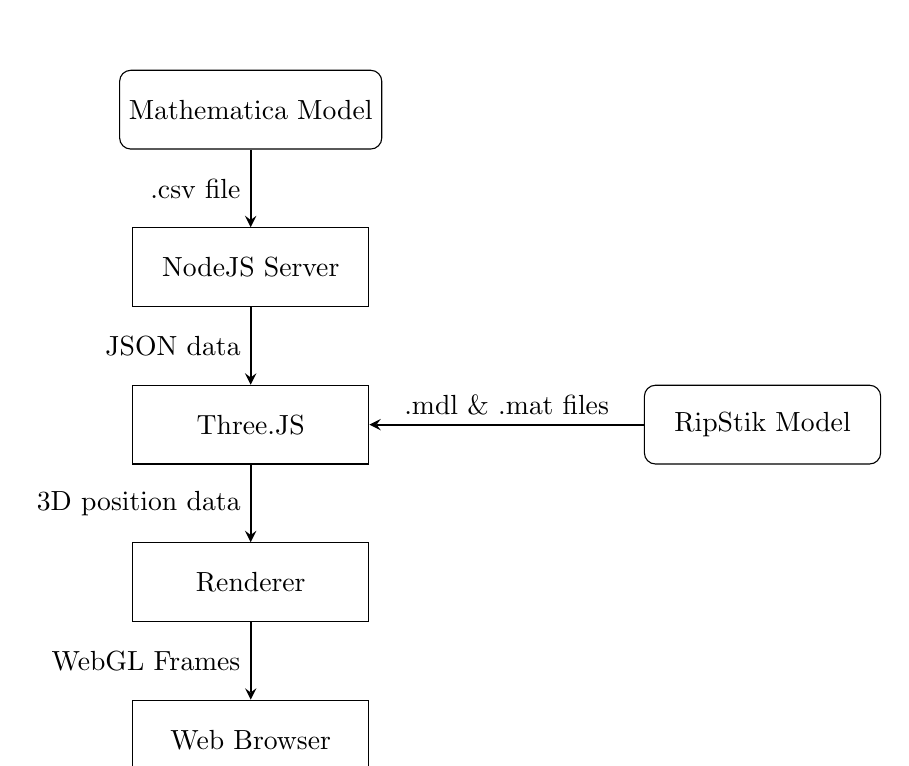
\begin{tikzpicture}[node distance=2cm]
				\node (WA) [startstop] {Mathematica Model};
				\node (Srvr) [process, below of=WA] {NodeJS Server};
				\node (Three) [process, below of=Srvr] {Three.JS};
				\node (Mdl) [startstop, right of=Three, xshift=4.5cm] {RipStik Model};
				\node (Rndr) [process, below of=Three] {Renderer};
				\node (Brwsr) [process, below of=Rndr] {Web Browser};

				\draw [arrow] (WA) -- node[anchor=east] {.csv file} (Srvr);
				\draw [arrow] (Srvr) -- node[anchor=east] {JSON data} (Three);
				\draw [arrow] (Mdl) -- node[anchor=south] {.mdl \& .mat files} (Three);
				\draw [arrow] (Three) -- node[anchor=east] {3D position data} (Rndr);
				\draw [arrow] (Rndr) -- node[anchor=east] {WebGL Frames} (Brwsr);
			\end{tikzpicture}
		\end{center}
	\caption{RipStik animation tool data flow summary}\label{fig:ThreeJsFlow}
	\end{figure}
\end{center}
The core of the application is ThreeJS, a javascript WebGL library that allows the 3D model to be loaded from a .mdl file (the set of 3D dimensional points that forms the shape) and .mat file (the colors/materials to be overlaid on the shape) then animated using rotations and translations in a standard Cartesian coordinate system.
\section{Design Methodology}
Throughout the project, an emphasis was placed on an iterative, test-driven design process. This testing involved both the use of smaller, well understood test cases and incremental unit tests in the context of the full system. 
The applicability of these smaller test cases stemmed from the use of the \textit{modular programming} paradigm, which will allow the same code to be used across a variety of different mechanical systems. 
A brief outline of the software tools used with this methodology will be followed by discussion of the core principals and importance of these concepts before formalizing the overarching process.
\subsection{Software Tools}
\subsubsection{Mathematica}
Due to the complex nature of the model and the large number of degrees of freedom needed to accurately model the behavior of the RipStik, a powerful symbolic computation tool is required to derive and manipulate the expressions. 
Mathematica was ultimately selected over other options such as Maple and the Matlab Symbolic toolbox due to the combination of robust symbolic and numeric computation features with easy to use visualization features for graphically displaying the various systems developed over the course of the project.
It also provided equivalent or better performance with thorough documentation and examples compared to competitors.
\subsubsection{Three.JS}
While all of the more simple visualizations were constructed directly in Mathematica, an external tool was constructed to animate the full RipStik system in a more attractive and visually intuitive manner. 
The application is javascript based and operated via the web browser, allowing the user to upload a .csv (comma separated value) file of numeric output from the RipStik simulation and returning an animation of the results on a 3 dimensional RipStik model. 
This allows easy validation of the results by inspection, particularly for complex motions where graphs of the angles and positions may not make the full system behavior immediately obvious.
The process used to generate these animations in the application is shown in Figure \ref{fig:ThreeJsFlow}.

%%Define the two block types and arrow type for our flow diagram
\tikzstyle{startstop} = [rectangle, rounded corners, minimum width=3cm, minimum height=1cm,text centered, draw=black, fill=white]
\tikzstyle{process} = [rectangle, minimum width=3cm, minimum height=1cm, text centered, draw=black, fill=white]
\tikzstyle{arrow} = [thick,->,>=stealth]
\begin{center}
	\begin{figure}[!htb]
		\begin{center}
			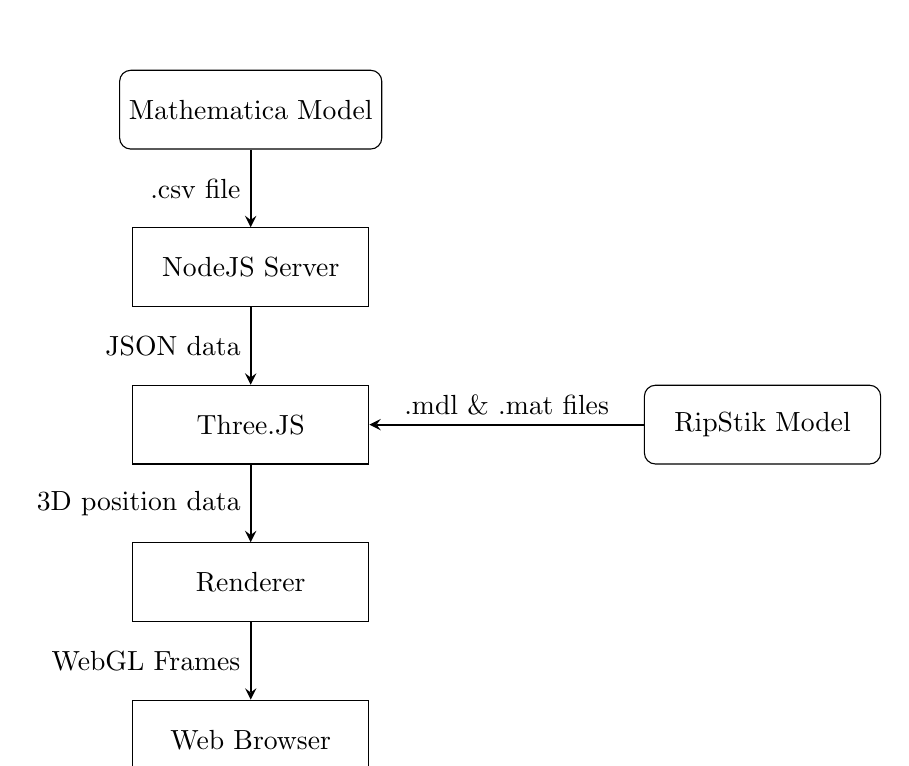
\begin{tikzpicture}[node distance=2cm]
				\node (WA) [startstop] {Mathematica Model};
				\node (Srvr) [process, below of=WA] {NodeJS Server};
				\node (Three) [process, below of=Srvr] {Three.JS};
				\node (Mdl) [startstop, right of=Three, xshift=4.5cm] {RipStik Model};
				\node (Rndr) [process, below of=Three] {Renderer};
				\node (Brwsr) [process, below of=Rndr] {Web Browser};

				\draw [arrow] (WA) -- node[anchor=east] {.csv file} (Srvr);
				\draw [arrow] (Srvr) -- node[anchor=east] {JSON data} (Three);
				\draw [arrow] (Mdl) -- node[anchor=south] {.mdl \& .mat files} (Three);
				\draw [arrow] (Three) -- node[anchor=east] {3D position data} (Rndr);
				\draw [arrow] (Rndr) -- node[anchor=east] {WebGL Frames} (Brwsr);
			\end{tikzpicture}
		\end{center}
	\caption{RipStik animation tool data flow summary}\label{fig:ThreeJsFlow}
	\end{figure}
\end{center}
The core of the application is ThreeJS, a javascript WebGL library that allows the 3D model to be loaded from a .mdl file (the set of 3D dimensional points that forms the shape) and .mat file (the colors/materials to be overlaid on the shape) then animated using rotations and translations in a standard Cartesian coordinate system.
\subsection{Modular Program Design}
The core principle of modular program design is to decompose the larger system design problem into small, independent modules\cite{Modular}.
An effective decomposition is done in such that the modules are have well defined inputs and outputs and can be tested independently, improving the flexibility of the application\cite{Modular}.
In designing the RipStik model, these modules are user created Mathematica functions, separated to each contain a complete, testable portion of the larger model.

Two alternate approaches were also considered but deemed unsuitable. Object Oriented design involves grouping related functionality and data, like parameters or variables, into larger "objects"\cite{ObjectOriented}.
This would provide similar compartmentalization \cite{ObjectOriented} but does not conform to the broader functional design of Mathematica \cite{MathematicaFunctional} and is less intuitive and legible for new users attempting to adopt code from the system. 

Alternately, a purely procedural approach would simply focus on laying out the set of commands sequentially in a single structure. 
This design would be more intuitive to new users and would likely improve initial development speed due to the lack of unit testing and reduced need for flexibility of the commands in sequence versus those implemented in independent modules.
Despite these benefits, this design was not selected since it would reduce the flexibility and testability of the system due to the purpose built nature of commands. 
This would make smaller test cases much more difficult to implement since each would be a completely independent code base with no shared functions outside of those central to Mathematica.
\subsection{Test Cases}
In order to validate each module during development, small test systems were developed. Each test system had to:
\begin{itemize}
\item Succinctly demonstrate the complete functionality of the module 
\item Be small and straightforward to minimize the time expended on setting up systems outside of the core RipStik model
\item Provide results that could be easily verified through simple visualizations and (where possible) published results
\end{itemize}
These test cases will be presented throughout the development of the model alongside the discussion of implementing each mathematical tool.
\subsection{Unit Testing}
In addition to the simple mechanical systems used to test each model, a test or set of tests was developed for the RipStik system to further validate that the given portion of the model was functioning as expected. These were designed to be as simple and easy to implement as possible while still testing the module as thoroughly as possible.
\subsection{Overall Process}
Together, modular program design, test cases and unit testing make up the core design process for each module as outlined in Figure \ref{fig:ProcessFlow}. These modules were then used to iteratively construct the overall RipStik model, adding functionality and testing incrementally for each mathematical tool applied.
\begin{center}
	\begin{figure}[!htb]
		\begin{center}
			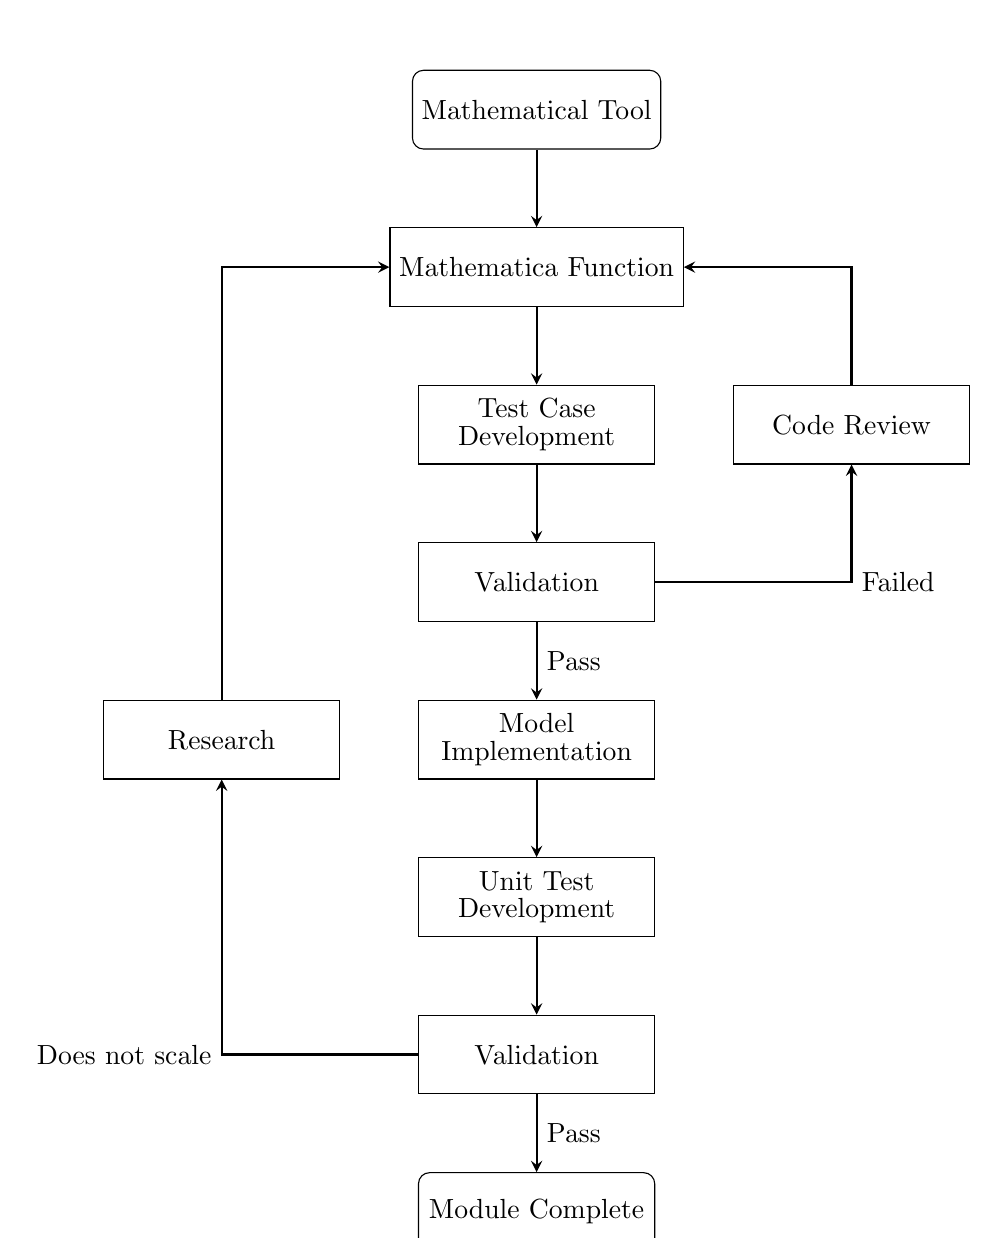
\begin{tikzpicture}[node distance=2cm]
				\node (math) [startstop] {Mathematical Tool};
				\node (code) [process, below of=math] {Mathematica Function};
				\node (testcase) [process, below of=code] {\shortstack{Test Case \\ Development}};
				\node (tcvalid) [process, below of=testcase] {Validation};
				\node (model) [process, below of=tcvalid] {\shortstack{Model \\ Implementation}};
				\node (unittest) [process, below of=model] {\shortstack{Unit Test \\ Development}};
				\node (utvalid) [process, below of=unittest] {Validation};
				\node (done) [startstop, below of=utvalid] {Module Complete};
				\node (research) [process, left of=model, node distance=4cm] {Research};
				\node (review) [process, right of=testcase, node distance=4cm] {Code Review};
				\draw [arrow] (math) -- (code);
				\draw [arrow] (code) -- (testcase);
				\draw [arrow] (testcase) -- (tcvalid);
				\draw [arrow] (tcvalid) -- node [anchor=west] {Pass}(model);
				\draw [arrow] (model) -- (unittest);
				\draw [arrow] (unittest) -- (utvalid);
				\draw [arrow] (utvalid) -- node [anchor=west] {Pass}(done);
				\draw [arrow] (utvalid) -| node [anchor=east] {Does not scale}(research);
				\draw [arrow] (research) |- (code);
				\draw [arrow] (tcvalid) -| node [anchor=west] {Failed}(review);
				\draw [arrow] (review) |- (code);
			\end{tikzpicture}
		\end{center}
	\caption{Design Process Summary Diagram}\label{fig:ProcessFlow}
	\end{figure}
\end{center}

\section{Model Development}
\subsection{Core Assumptions}

With the mathematical concepts and software tools clearly defined, a number of assumptions need to be made for the RipStik model.
\par
The RipStik will be treated as 5 separate bodies; the torsion rod (1), front plate (2), back plate (3), front caster (4), and back caster (5).

\begin{figure}[!htb]
	\centering
	\minipage{0.7\textwidth}
	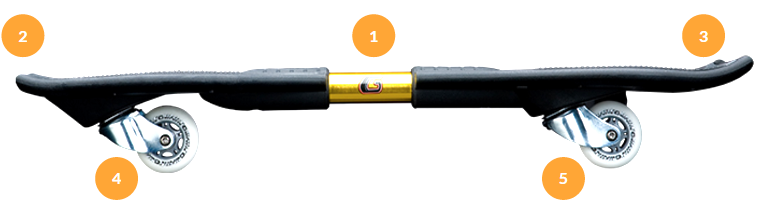
\includegraphics[width=\linewidth]{RipStikModel.png}
	\caption{Image depicting the 5 separate bodies of the RipStik}\label{fig:RipStikModel}
	\endminipage
\end{figure}  

Difficulties associated with accurately modeling the complex geometry of the RipStik led to simplifying assumptions being made for the shapes of the 5 separate bodies.
The front and back plates were treated as rectangular prisms while defining inertia tensors for the bodies, and the inertia tensors for the wheels were combined with the casters. 
Additionally, the casters were treated as skates to emulate the constrained motion of the casters while simplifying the overall system dynamics.
\par
The spring in the torsion rod was omitted since it is not a critical component of the RipStik and will add unnecessary complexity to the system in the form of kinetic energy.
Friction between the bodies of the RipStik was omitted, since it would be difficult to accurately model and does not have a significant impact on the general dynamics of the system.

\subsection{Coordinate Systems}

The initial focus for developing a mathematical model of the RipStik was placed on determining the number of degrees of freedom in the system. 
A coordinate system was defined, assumptions were made, and Euler angles were applied to said coordinate system so that all degrees of freedom could be explicitly defined.
\par
A body-fixed coordinate system for the RipStik was developed such that the origin was placed at the center of the torsion bar. The X-Y plane will be parallel with the RipStik Deck at rest with no torsion applied.
The +X direction points through the torsion bar towards the front plate, and the Y axis is defined perpendicular to the X axis. The Z axis is normal to the X-Y plane, with +Z pointing upwards. The +Y direction is defined based on the right hand rule.

With the coordinate system defined, Euler angles were implemented into the system to represent the roll ($\alpha$), pitch ($\psi$), and yaw ($\theta$).
\par
The roll angles ($\alpha$) describe the rotation of the deck platform about the X-axis. There will be two roll angles on the RipStik, the first on the front platform ($\alpha_{fp}$) and the second on the rear platform ($\alpha_{bp}$).
\par
The pitch angle ($\psi$) is the angle that the wheels make, offset by the caster angle ($\phi$). This represents a rotation about the Y axis. The wheels are completely unbounded in their ability to rotate, and can pivot through [0, 2$\pi$].
\par
The yaw angle ($\theta$) was represented by a moment taken around the Z-axis (right hand rule applied). There will be two yaw angles on the RipStik, the first on the front caster ($\theta_{fc}$), and the second on the back caster ($\theta_{bc}$).

The RipStik has ten degrees of freedom represented by [X, Y, Z, $\alpha$, $\psi$, $\theta$, $\alpha_{fp}$, $\alpha_{bp}$, $\theta_{fc}$, $\theta_{bc}$].

\subsubsection{Test Case - Caster Rotation}

In order to validate the selected coordinate system, a test case was conducted for RipStik. This was done by analyzing the behavior of the caster as it went through a full revolution (2$\pi$ radians).
The output for the X,Y, and Z positions were plotted as a function of the casters rotation as seen in Figure \ref{fig:CasterWheel2DTest}.

\begin{figure}[!htb]
	\centering
	\minipage{0.7\textwidth}
	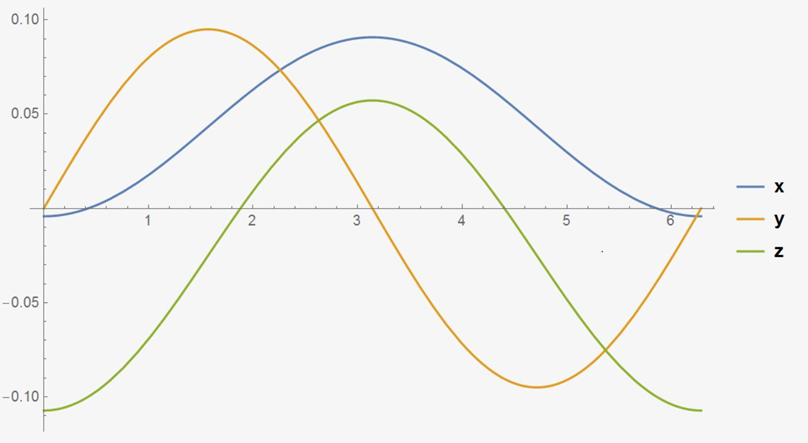
\includegraphics[width=\linewidth]{CasterWheel2DTest.png}
	\caption{The X ,Y, and Z positions of the caster were plotted as a function of the caster angle (in radians)}\label{fig:CasterWheel2DTest}
	\endminipage
\end{figure} 

With the two-dimensional plot completed, a three-dimensional plot was created to ensure that the casters obeyed the caster orientation that was previously defined, and can be seen in Figure \ref{fig:CasterWheel3DTest}.

\begin{figure}[!htb]
	\centering
	\minipage{0.7\textwidth}
	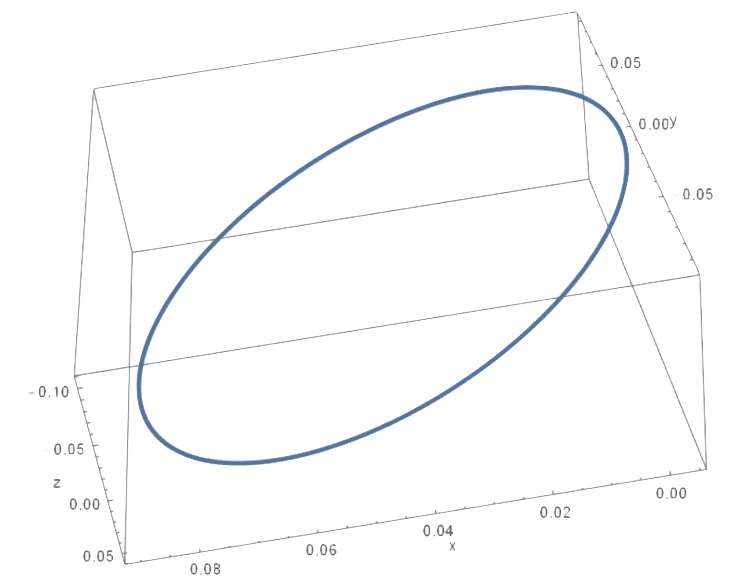
\includegraphics[width=\linewidth]{CasterWheel3DTest.png}
	\caption{The X ,Y, and Z positions of the caster were plotted as a function of the caster angle (in radians) on a three-dimensional plot}\label{fig:CasterWheel3DTest}
	\endminipage
\end{figure} 

\subsubsection{Model Implementation}

With the test case completed and verified, the coordinate system for the RipStik model was verified for each degree of freedom in the system. 
This was completed by taking applying the output from Mathematica into the ThreeJS based visualization tool.

\textbf{INCLUDE SCREENSHOT FROM ANIMATION?}
\subsubsection{Validation}

Each degree of freedom in the system behaved as expected. 
Therefore, the selected coordinate system was correct, and the equations of motion can be developed.

\subsection{Equations of Motion}

To develop the equations of motion for the RipStik, the Lagrangian needs to be clearly developed. Given Equation \ref{eq:Lagrange}, it is necessary to break down the components of kinetic and potential energies in the system.

The kinetic energy in the system is composed of translational and rotational components.
The Translational Kinetic Energy (TKE) is modeled in the following fashion:

\begin{equation}
\label{eq:TKE}
\text{TKE} = \frac{1}{2}{\text{m}}{\lvert \lvert {\dot{\text{r}}^2} \rvert \rvert}
\end{equation}

In Equation \ref{eq:TKE}, m represents the mass of the body and $\dot{r}$ represents the translational velocity of the body.
\par
The Rotational kinetic energy (RKE) is modeled in the following fashion:

\begin{equation}
\label{eq:RKE}
\text{RKE} = \frac{1}{2}({\text{I}}{\omega(t)})^T\omega(t)
\end{equation}

In Equation \ref{eq:RKE}, I represents the inertia tensor of the body, and $\omega(t)$ represents the angular velocity of the body.

Finding the angular velocity for the body requires the following process. First, $\hat{\omega(t)}$ is solved for using Equation \ref{eq:omegahat}.

\begin{equation}
\label{eq:omegahat}
\hat{\omega}(t)=R^T(t)\dot{R(t)}
\end{equation}

Equation \ref{eq:omegahat} generates a 3x3 skew-symmetric matrix. The angular velocity is then a column vector composed of 3 elements from $\hat{\omega}(t)$, seen in Equation \ref{eq:omega}.

\begin{equation}
\label{eq:omega}
\omega(t)=\begin{bmatrix}
\hat{\omega}(t)[3,2] \\
\hat{\omega}(t)[1,3] \\
\hat{\omega}(t)[2,1]\\
\end{bmatrix}
\end{equation}

The potential energy in the system is composed of only Gravitational Potential Energy (GPE). This is modelled by Equation \ref{eq:GPE}.

\begin{equation}
\label{eq:GPE}
\text{GPE} = {\text{m}}{\text{g}}{\text{h}}
\end{equation}

In Equation \ref{eq:GPE}, m represents the mass of the body and h represents the height of the body relative to the ground plane.

With the kinetic and potential energies explicitly defined, the Lagrangian can be written as follows:

\begin{equation}
L= \frac{1}{2}{\text{m}}{\lvert \lvert {\dot{\text{r}}^2} \rvert \rvert} + \frac{1}{2}({\text{I}}{\omega(t)})^T\omega(t) - {\text{m}}{\text{g}}{\text{h}}
\end{equation}

The explicit Lagrangian can then be applied to the Euler-Lagrange equations do develop the ten unconstrained equations of motion for each degree of freedom using Equation \ref{eq:UEOM}.

\subsubsection{Test Case - Uncontrolled Inverted Pendulum}\label{sec:testcaseip}

The equations of motion were validated using an unconstrained system. A pendulum  attached to a moving cart with an initial position pointing upwards was modeled using Lagrangian mechanics. 
The mass of the cart is defined as $m_{1}$ and the mass of the pendulum is defined as $m_{2}$. 
The set up of the coordinate system can be seen in figure \ref{fig:pendulumcart}.

\begin{figure}[!htb]
	\centering
	\minipage{0.5\textwidth}
	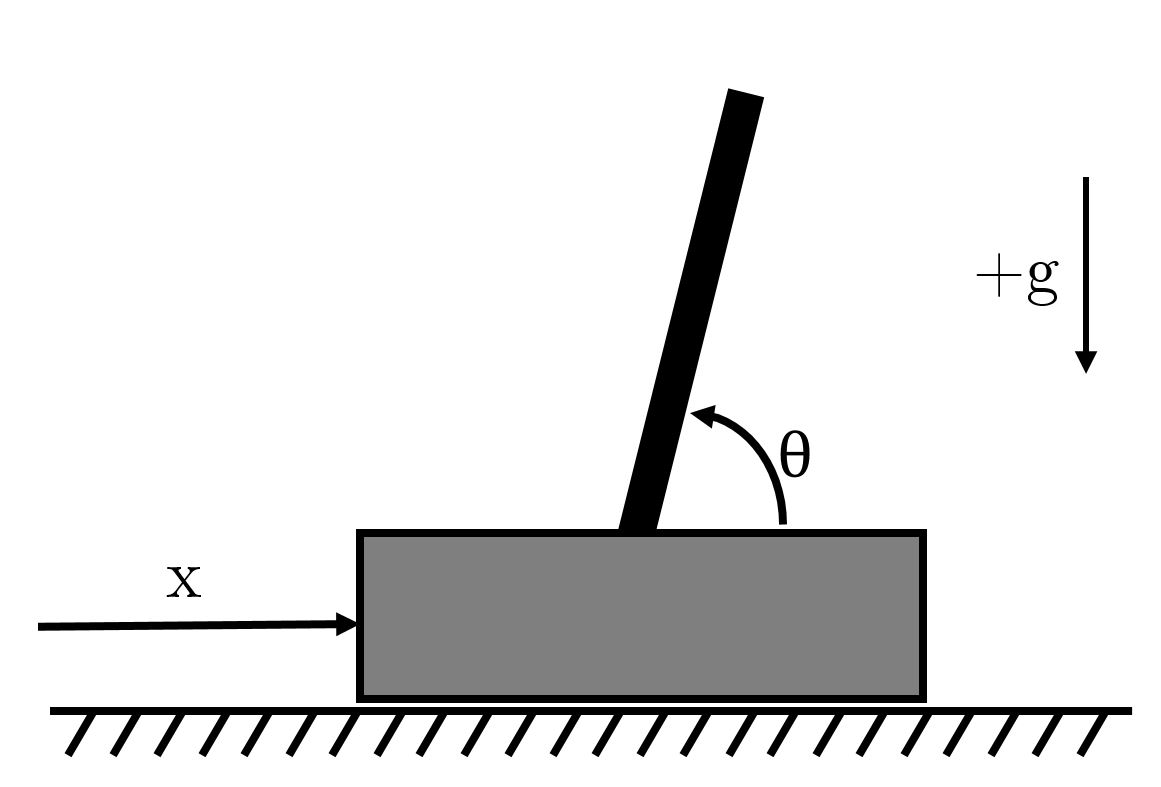
\includegraphics[width=\linewidth]{pendulumcart}
	\caption{Model set-up for the pendulum cart example}\label{fig:pendulumcart}
	\endminipage
\end{figure} 

The Lagrangian for the system is seen in Equation \ref{eq:CartLagrange}.

\begin{equation}
\label{eq:CartLagrange}
L = \frac{1}{2}m_{1}X'(t)^2+\frac{1}{2}m_{2}(2gL\sin\theta(t)+2L^2\theta'(t)^2-2L\sin\theta(t)\theta'(t)X'(t)+X'(t)^2) 
\end{equation}

With the Lagrangian developed, the equations of motion were solved for the two degrees of freedom (X(t), $\theta(t)$):

\begin{equation}
Lm_{2}\cos\theta(t)\theta'(t)^2+Lm_{2}\sin\theta(t)\theta''(t)-(m_{1}+m_{2})X''(t) = 0
\end{equation}

\begin{equation}
Lm_{2}(g\cos\theta(t)-2L\theta''(t)+\sin\theta(t)X''(t)) = 0
\end{equation}

With these equations of motion, it was confirmed that the pendulum reacted as expected when the cart moved positions.

\subsubsection{Model Implementation}

With the test case complete, the equations of motion were tested on the RipStik model. A Z coordinate in the center of the torsion rod of the RipStik was fixed.
An initial roll angle of 45 degrees was applied to the front plate ($\alpha_{fp}$), and an initial roll angle of -45 degrees was applied to the back plate ($\alpha_{bp}$). 

\subsubsection{Validation}

When the model implementation was tested with the conditions specified previously, the RipStik behaved as expected. 
The front and back plated experienced an oscillating motion between 45 and -45 degrees, with the casters rotating between 45 and -45 degrees. 
Plots for roll of the front plate ($\alpha_{fp}$), roll of the back plate ($\alpha_{bp}$), yaw of the front caster ($\theta_{fc}$), and yaw of the back caster ($\theta_{bc}$) were plotted to ensure that the motion of the Ripstik aligned with the expected behaviour.

\begin{figure}[!htb]
	\centering
	\minipage{0.4\textwidth}
	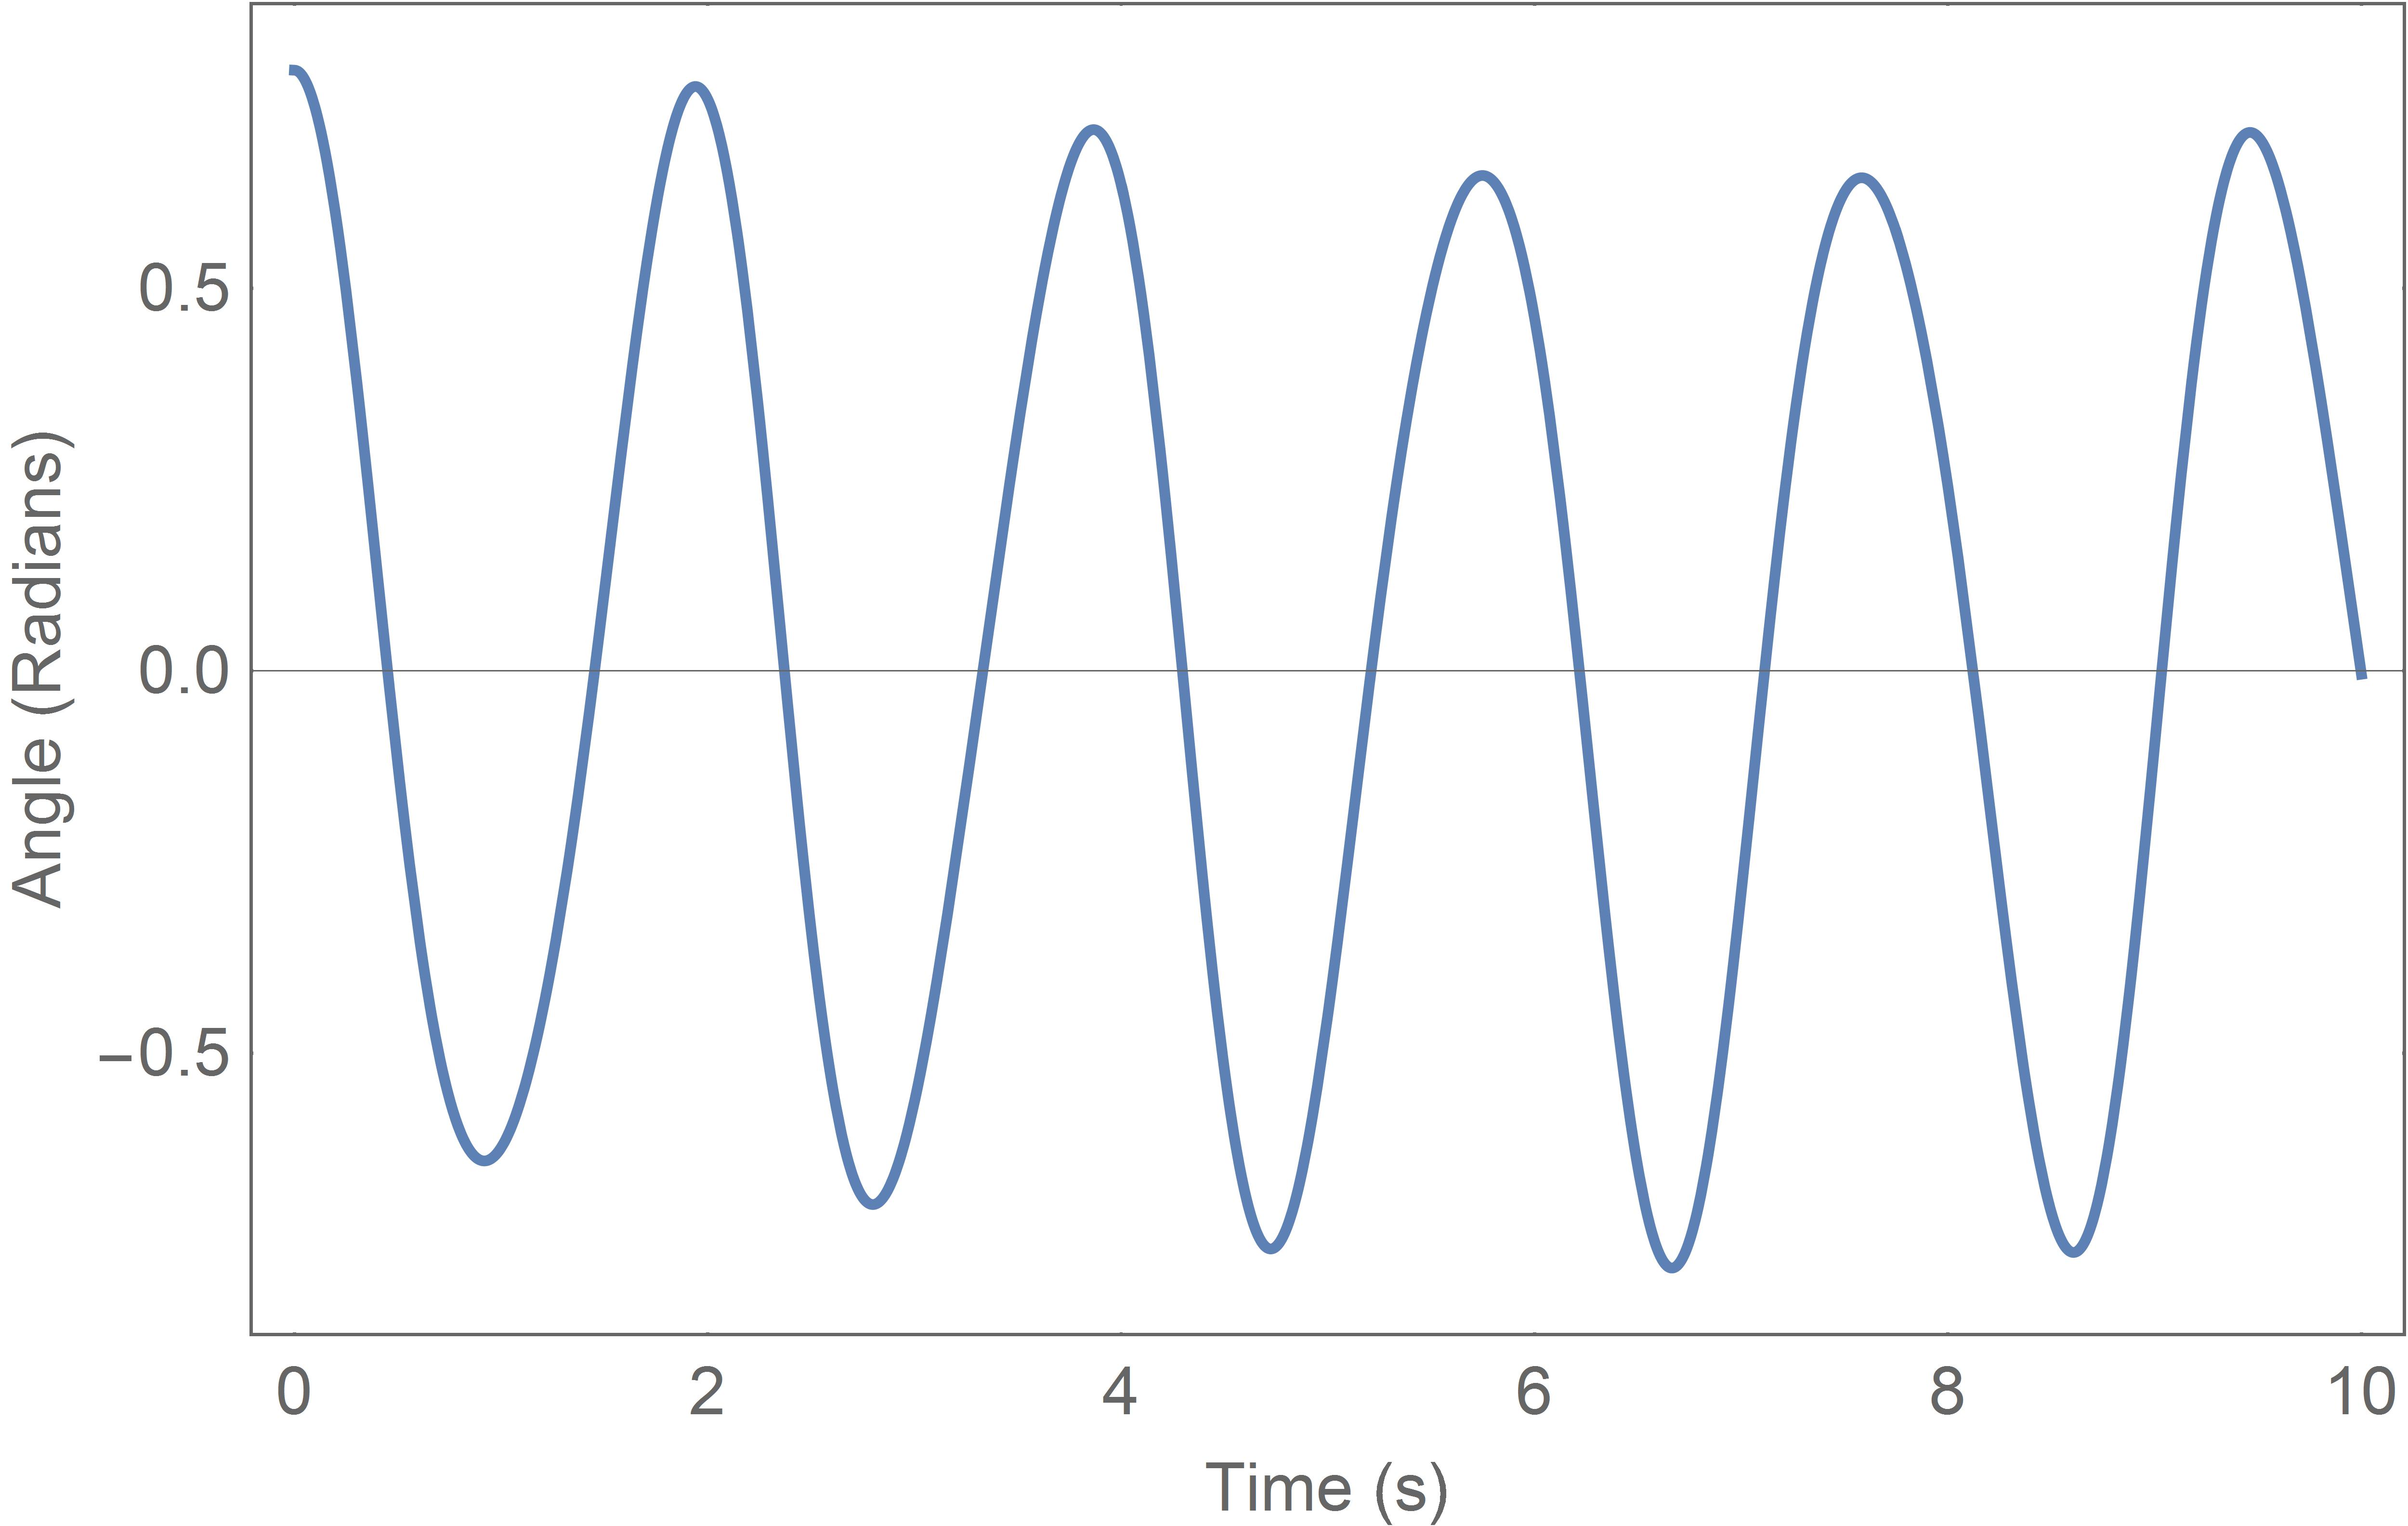
\includegraphics[width=\linewidth]{alphafp}
	\endminipage\hspace{1em}%
	\minipage{0.4\textwidth}
	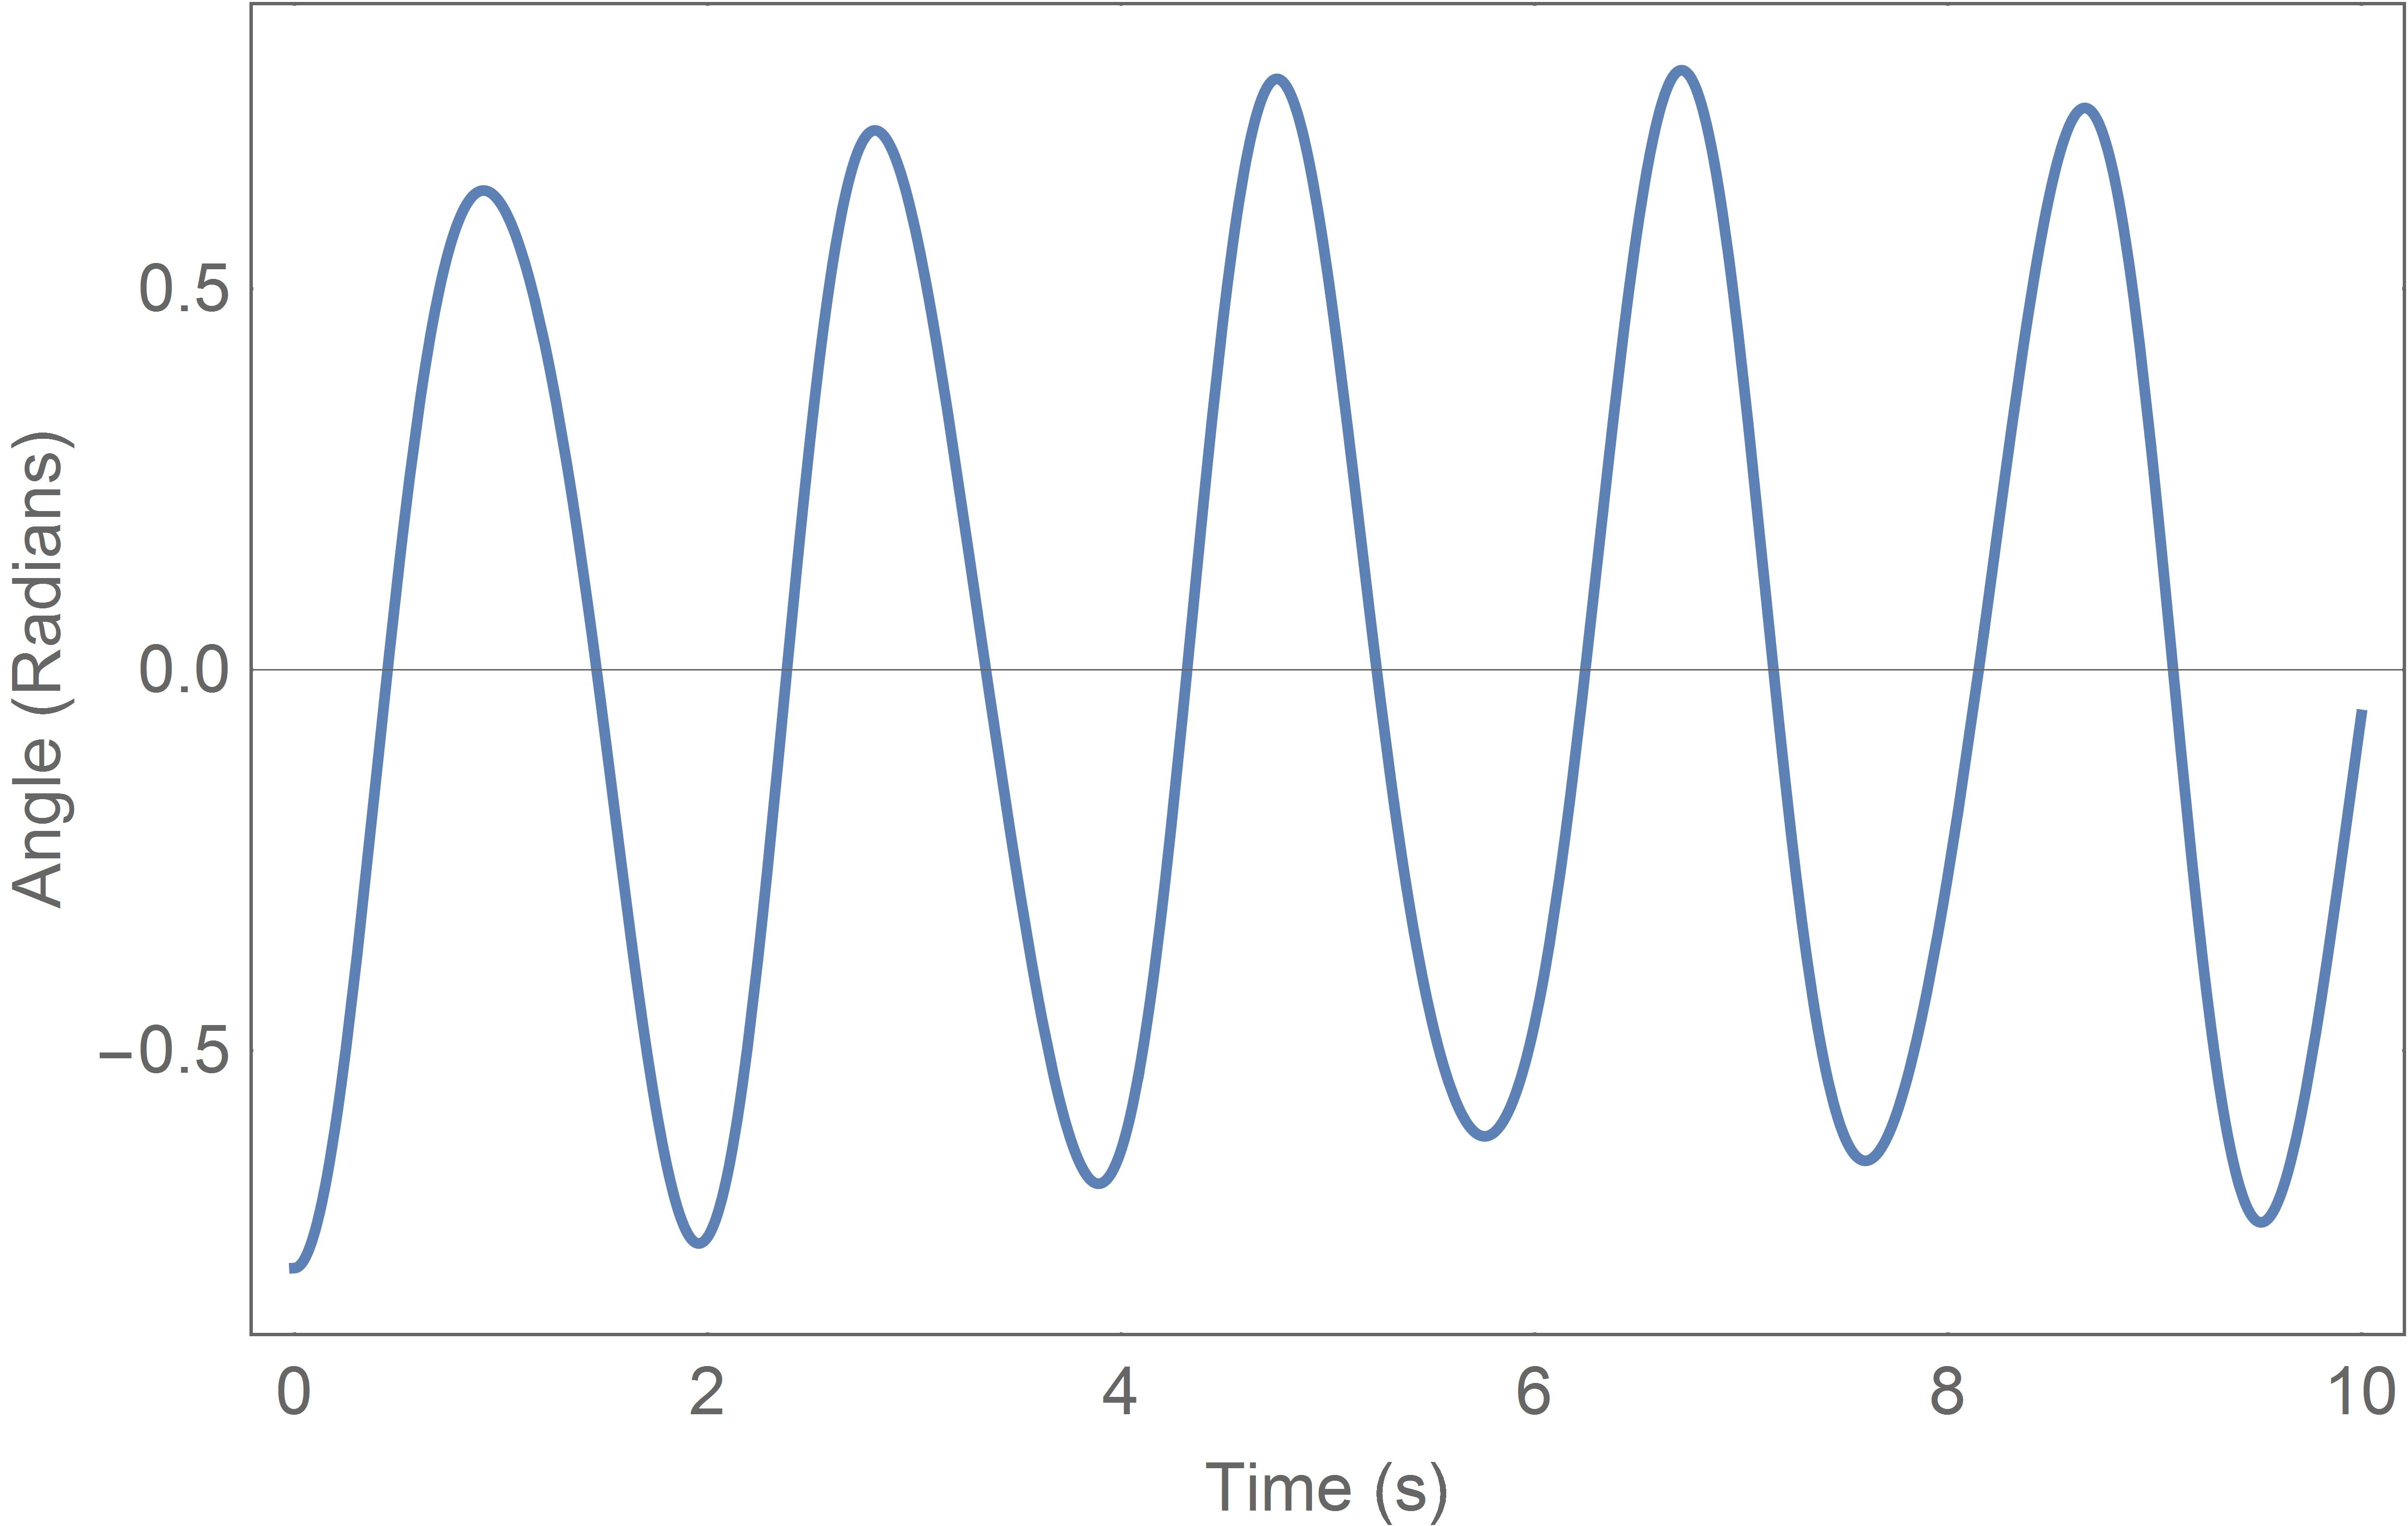
\includegraphics[width=\linewidth]{alphabp}
	\endminipage
	\caption{Roll of front plate ($\alpha_{fp}$) and back plate ($\alpha_{bp}$)}
	\label{fig:plates}
\end{figure}

\begin{figure}[!htb]
	\centering
	\minipage{0.4\textwidth}
	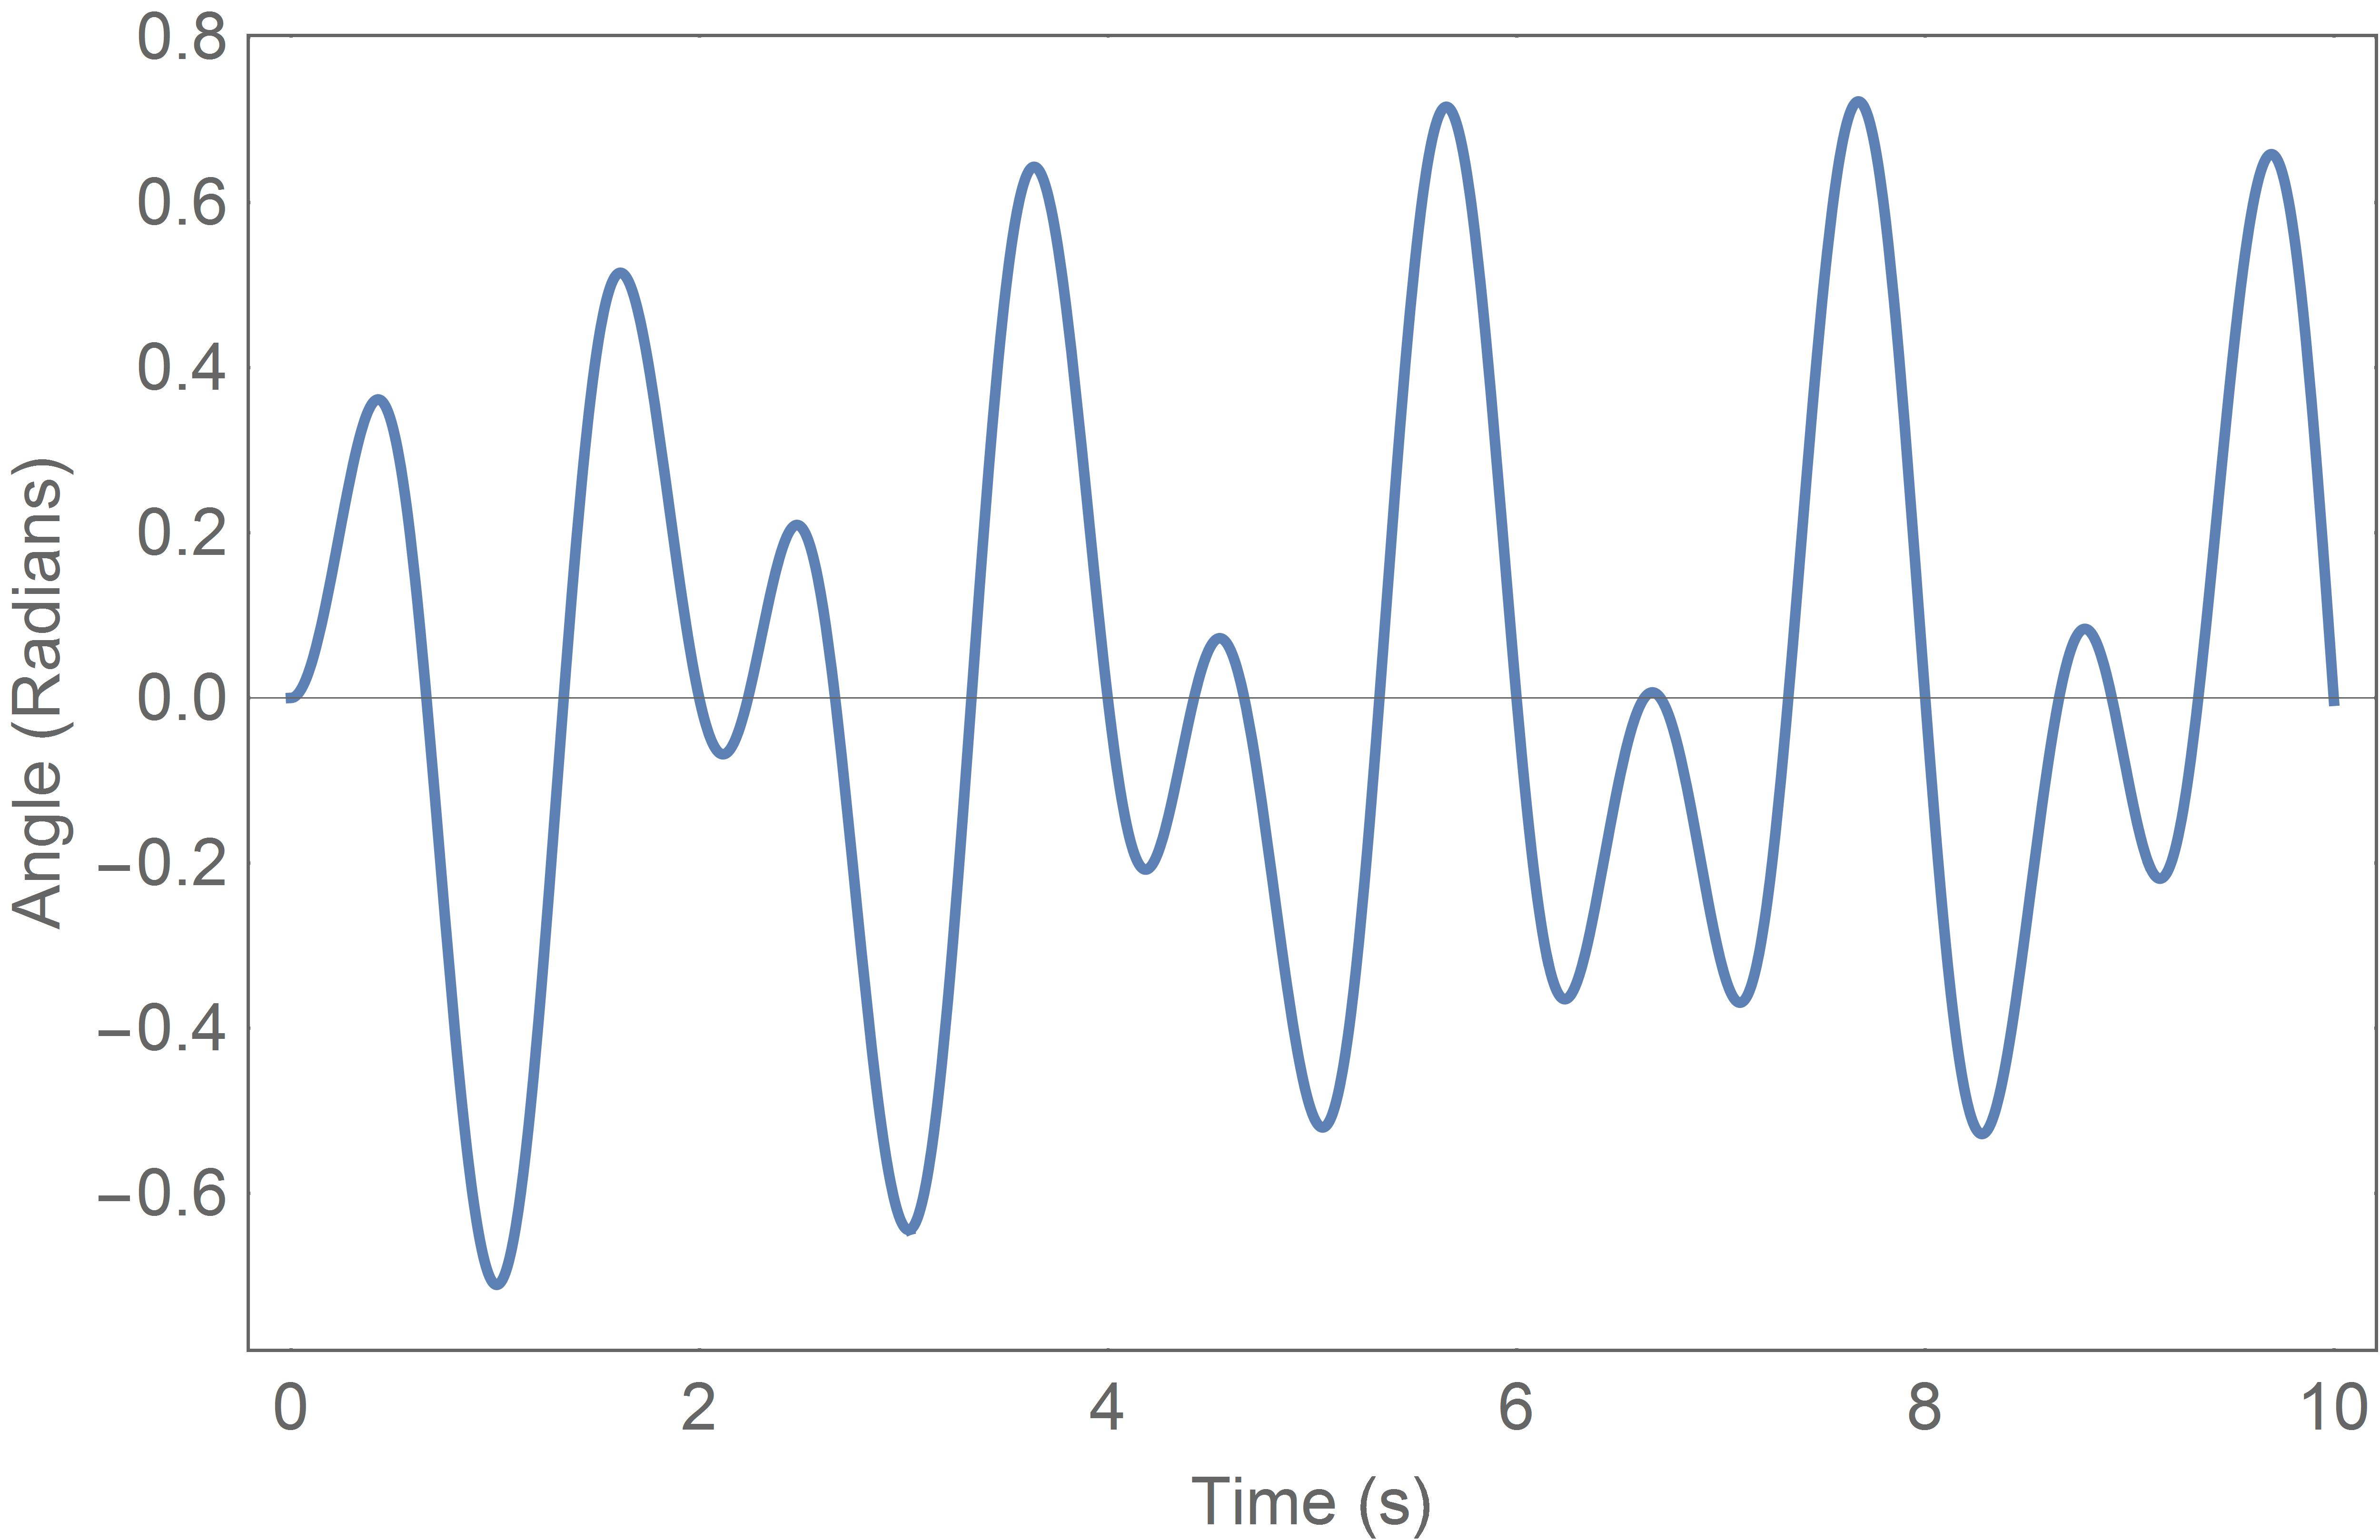
\includegraphics[width=\linewidth]{thetafc}
	\endminipage\hspace{1em}%
	\minipage{0.4\textwidth}
	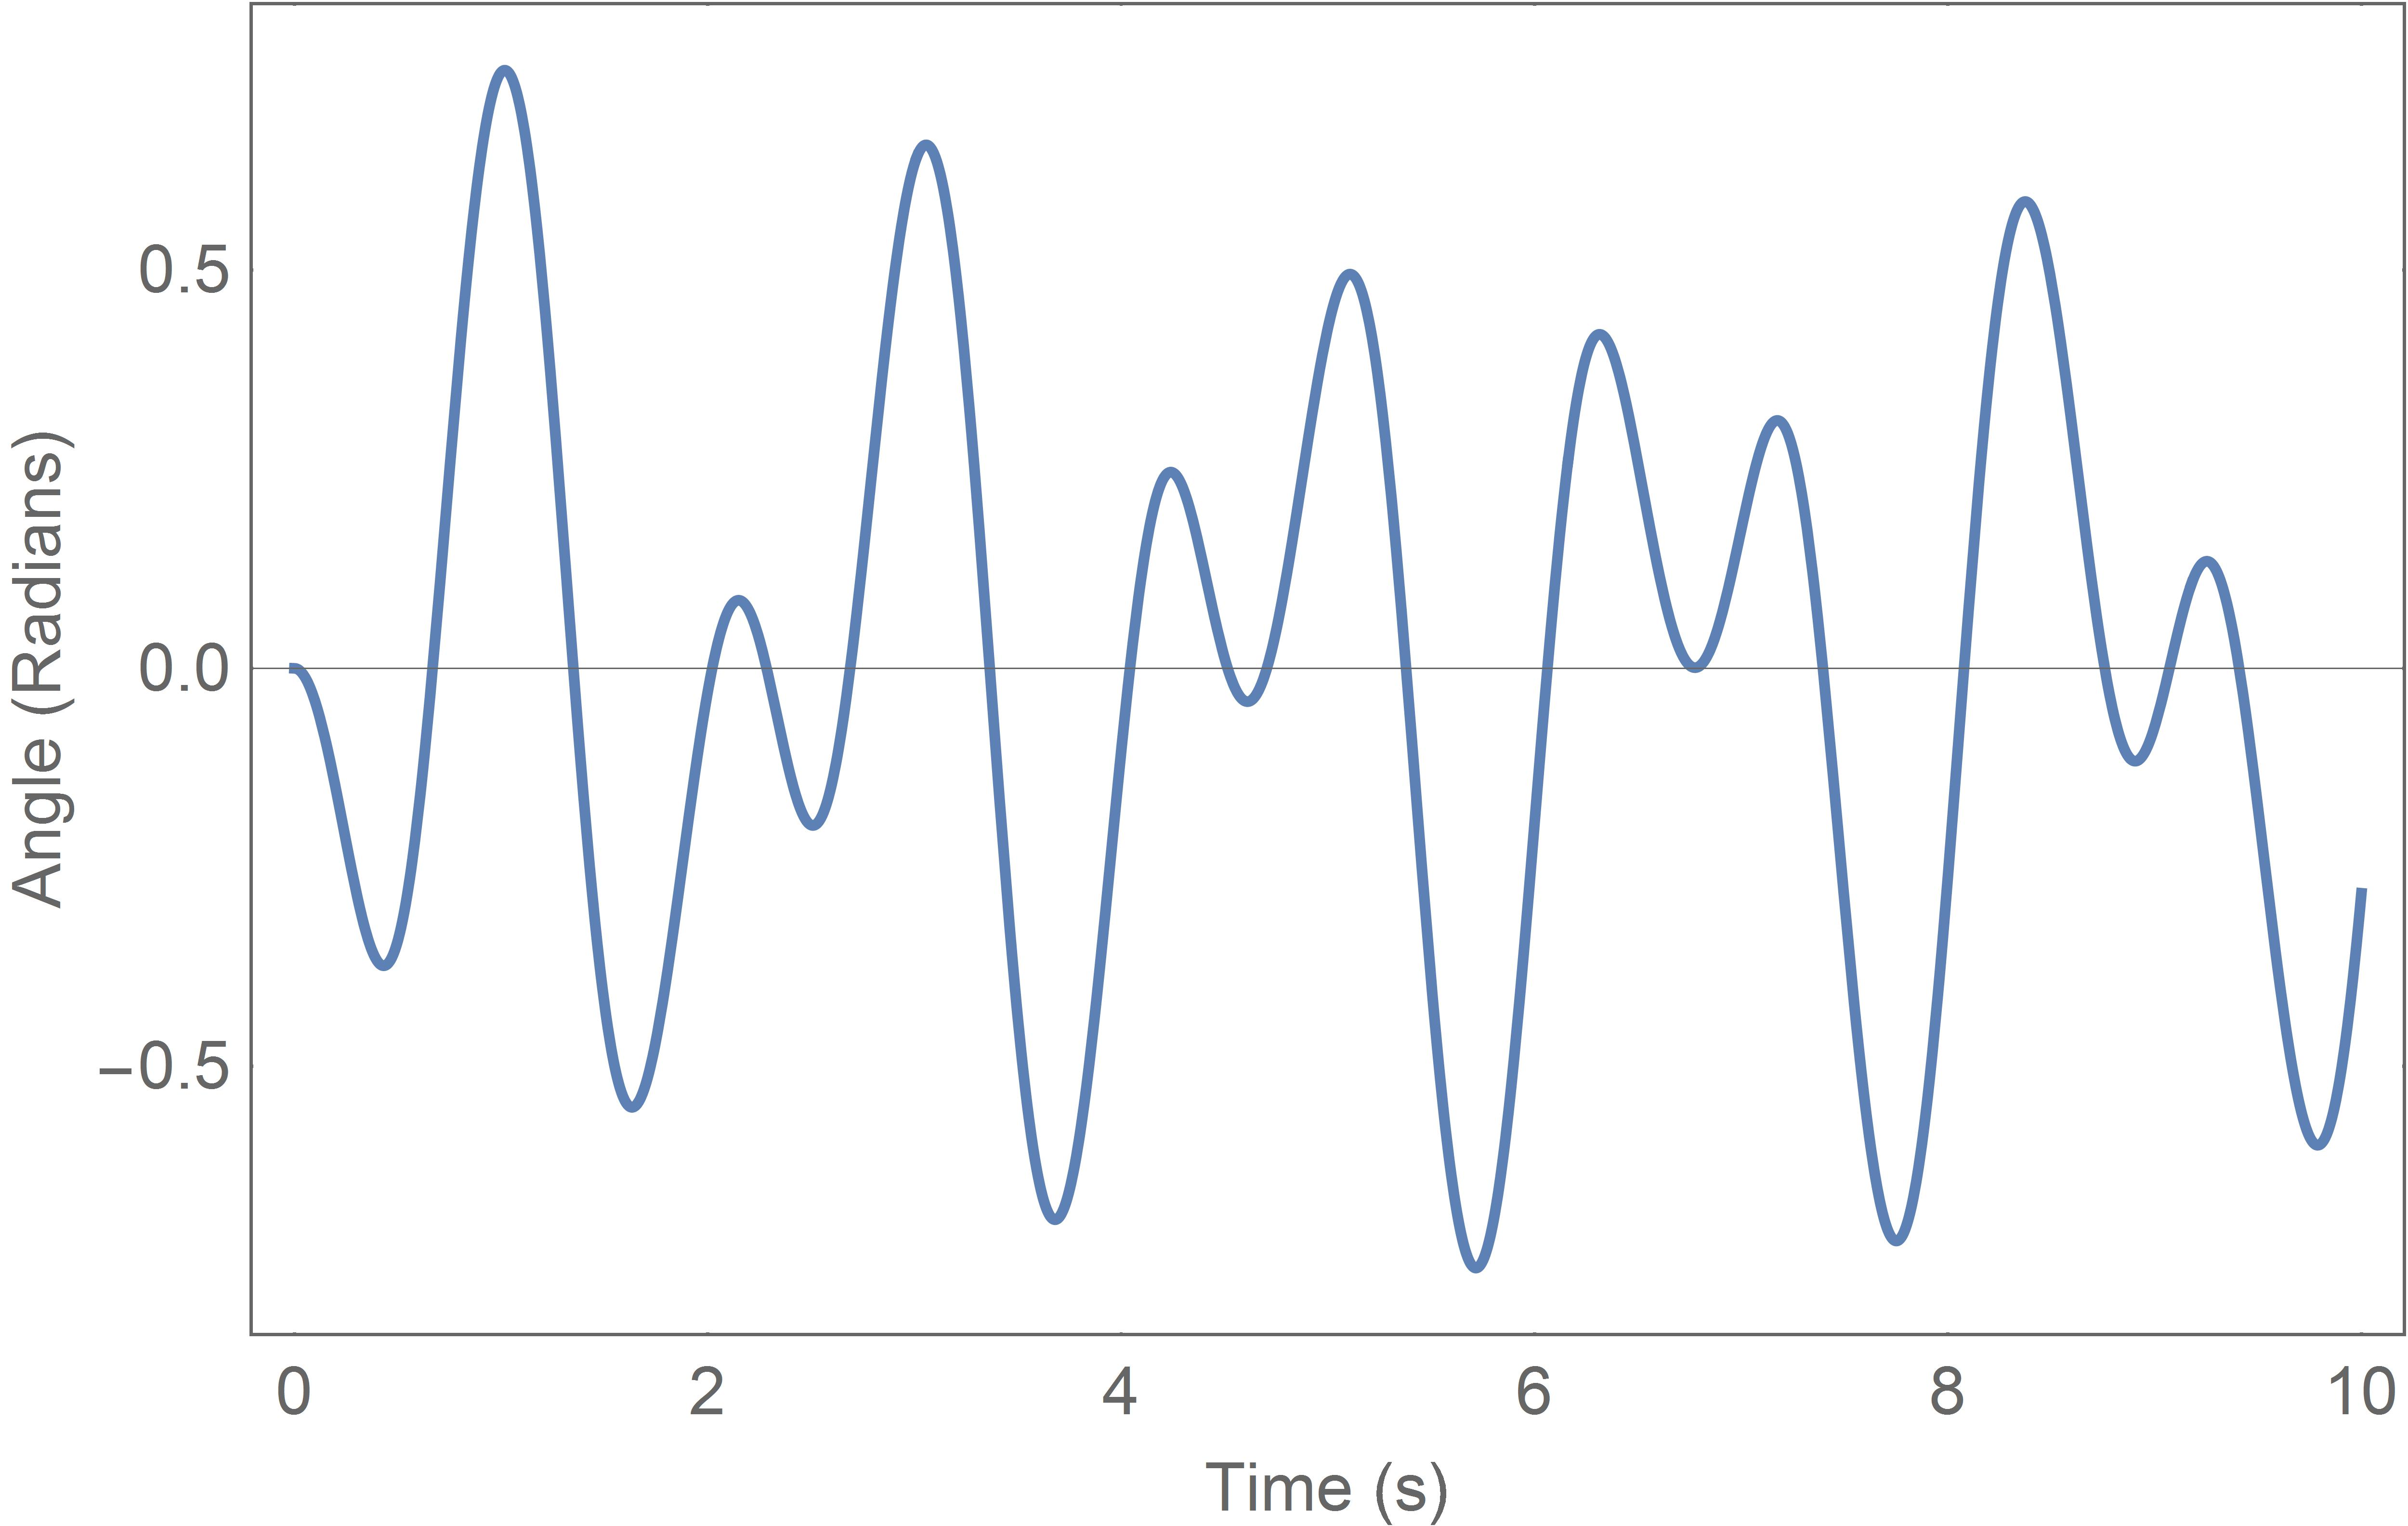
\includegraphics[width=\linewidth]{thetabc}
	\endminipage
	\caption{Yaw of front caster ($\theta_{fc}$) and back caster ($\theta_{bc}$)}
	\label{fig:casters}
\end{figure}

Since the plates and casters both experienced oscillations approximately between 45 and -45 degrees, it can be confirmed that the equations of motion for the RipStick were accurate.

An accurate visualization of the Ripstik was produced to model the motion and the two extreme positions of the RipStik can be seen in figure \ref{fig:RipStikModel1}.

\begin{figure}[!htb]
	\centering
	\minipage{0.4\textwidth}
	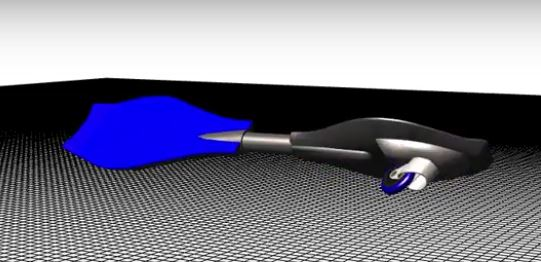
\includegraphics[width=\linewidth]{oneswing}
	\endminipage\hspace{1em}%
	\minipage{0.42\textwidth}
	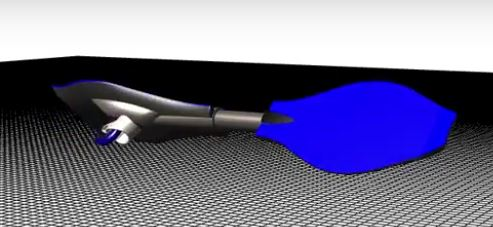
\includegraphics[width=\linewidth]{twoswing}
	\endminipage
	\caption{Two extreme positions of the RipStik motion}
	\label{fig:RipStikModel1}
\end{figure}

\subsection{Nonholonomic Constraints}

With the unconstrained equations of motion validated, nonholonomic constraints were implemented into the system. 
The constraints were defined such that the wheels could not slide laterally or lift off the ground. 
This represented a total of four constraint forces which were implemented using Lagrange multipliers.
Three different methods were explored when trying to solve for the nonholonomic constraints: symbolically inverting the matrices, representing the constraints as a system of linear equations $(Ax=B)$, and numeric integration.

\paragraph{Symbolic Matrix Inversion}\mbox{}\\
The initial method explored involved symbolically inverting matrices in Mathematica. First, the acceleration terms in the equations of motion were isolated for, which could then be substituted into the derivatives of the nonholonomic constraint equations, seen in Equation \ref{eq:SMI}.

\begin{equation}
\label{eq:SMI}
\Omega \ddot{q} = -\Omega G_{jk}^{-1}\Gamma_{jkl} \dot{q}^k\dot{q}^l + \Omega G_{jk}^{-1} \Omega ^T \lambda
\end{equation}

This is an intuitive approach from a linear algebra perspective; however, it is computationally impossible on large scale systems. 
When trying to solve for the acceleration terms, the computer's RAM completely fills and Mathematica is forced to abandon the calculation.

%%%%%%%%%%%%%%%%%%%%%%%%%%%%%%%%%%%%%%%%%%%%%%%%%%%
%%%%%%
%%%%%% MORE SPECIFIC ABOUT WHY RAM FILLS IE DETERMINANTS. Double check equation, the coeffs look a little fucky?
%%%%%%
%%%%%%%%%%%%%%%%%%%%%%%%%%%%%%%%%%%%%%%%%%%%%%%%%%%
\paragraph{System of Linear Equations $(Ax=B)$}\mbox{}\\
The next method attempted required taking the matrix inversion and representing it as a system of linear equations of the form Ax=b. 
In this equation, A is a square matrix and b is a column vector.
This allows Mathematics more flexibility to internally choose from three different approaches for isolating the desired results, using Laplace cofactor expansion, Bareiss method of division-free row reduction, and standard row reduction for computing determinants \cite{linearsolve}.
Bareiss method of division-free row reduction allows for the computation of determinants without introducting fractions \cite{bareiss}.
\par
At this point, all symbolic constants were replaced with with measured values to further simplify computations.
Using this method, the accelerations were solved in the equations of motion, but trying to find the lagrange multipliers in the second system exceeded computation times.

\paragraph{Numeric Integration}\mbox{}\\
The final method analyzed involved solving the system numerically.
Using this method, Equations \ref{eq:CFE} and \ref{eq:CV} can remain in their initial form.
Numeric integration functions can then be applied to approximate the result of the system of differential equations and ultimately produce output from the model.
A drawback associated with this method is that it can be a difficult process requiring careful tuning of numerical integrators and ultimately does not give explicit equations for the constraints.

\subsubsection{Test Case - Rolling Wheel}\label{sec:testcaserw}

Prior to implementing the three methods in the RipStik system, a simple model of a rolling wheel was used to validate the different approaches. For nonholonomic constraints, a code was developed and tested on the simple example of a wheel that rolls without slipping.
No slip constraints are considered to be nonholonomic, and the output can be easily compared to published results.
The configuration space for the rolling wheel consists of [X(t), Y(t), $\theta(t)$, $\phi(t)$].
The Lagragian for the system is seen in Equation \ref{eq:rollingdicks}.

\begin{equation}
\label{eq:rollingdicks}
L=\frac{1}{2}(mX'(t)^2+mY'(t)^2+Jroll\theta'(t)^2+Jspin\phi'(t)^2)
\end{equation}

With the Lagrangian developed, it was then applied to the Euler-Lagrange equations to provide the equations of motion, seen in equations \ref{eq:Xroll}, \ref{eq:Yroll}, \ref{eq:thetaroll}, and \ref{eq:phiroll}.

\begin{equation}
\label{eq:Xroll}
-mX''(t)=0
\end{equation}

\begin{equation}
\label{eq:Yroll}
-mY''(t)=0
\end{equation}

\begin{equation}
\label{eq:thetaroll}
-Jroll\theta''(t)=0
\end{equation}

\begin{equation}
\label{eq:phiroll}
-Jspin\phi''(t)=0
\end{equation}

Plots were then created to confirm that the rolling wheel's equations of motion with nonholonomic constraints behaved as expected.
The X and Y positions of the rolling wheel were modeled on a parametric plot, while $\theta$ and $\phi$ were modeled on a standard plot.

\begin{figure}[!htb]
	\centering
	\minipage{0.2\textwidth}
	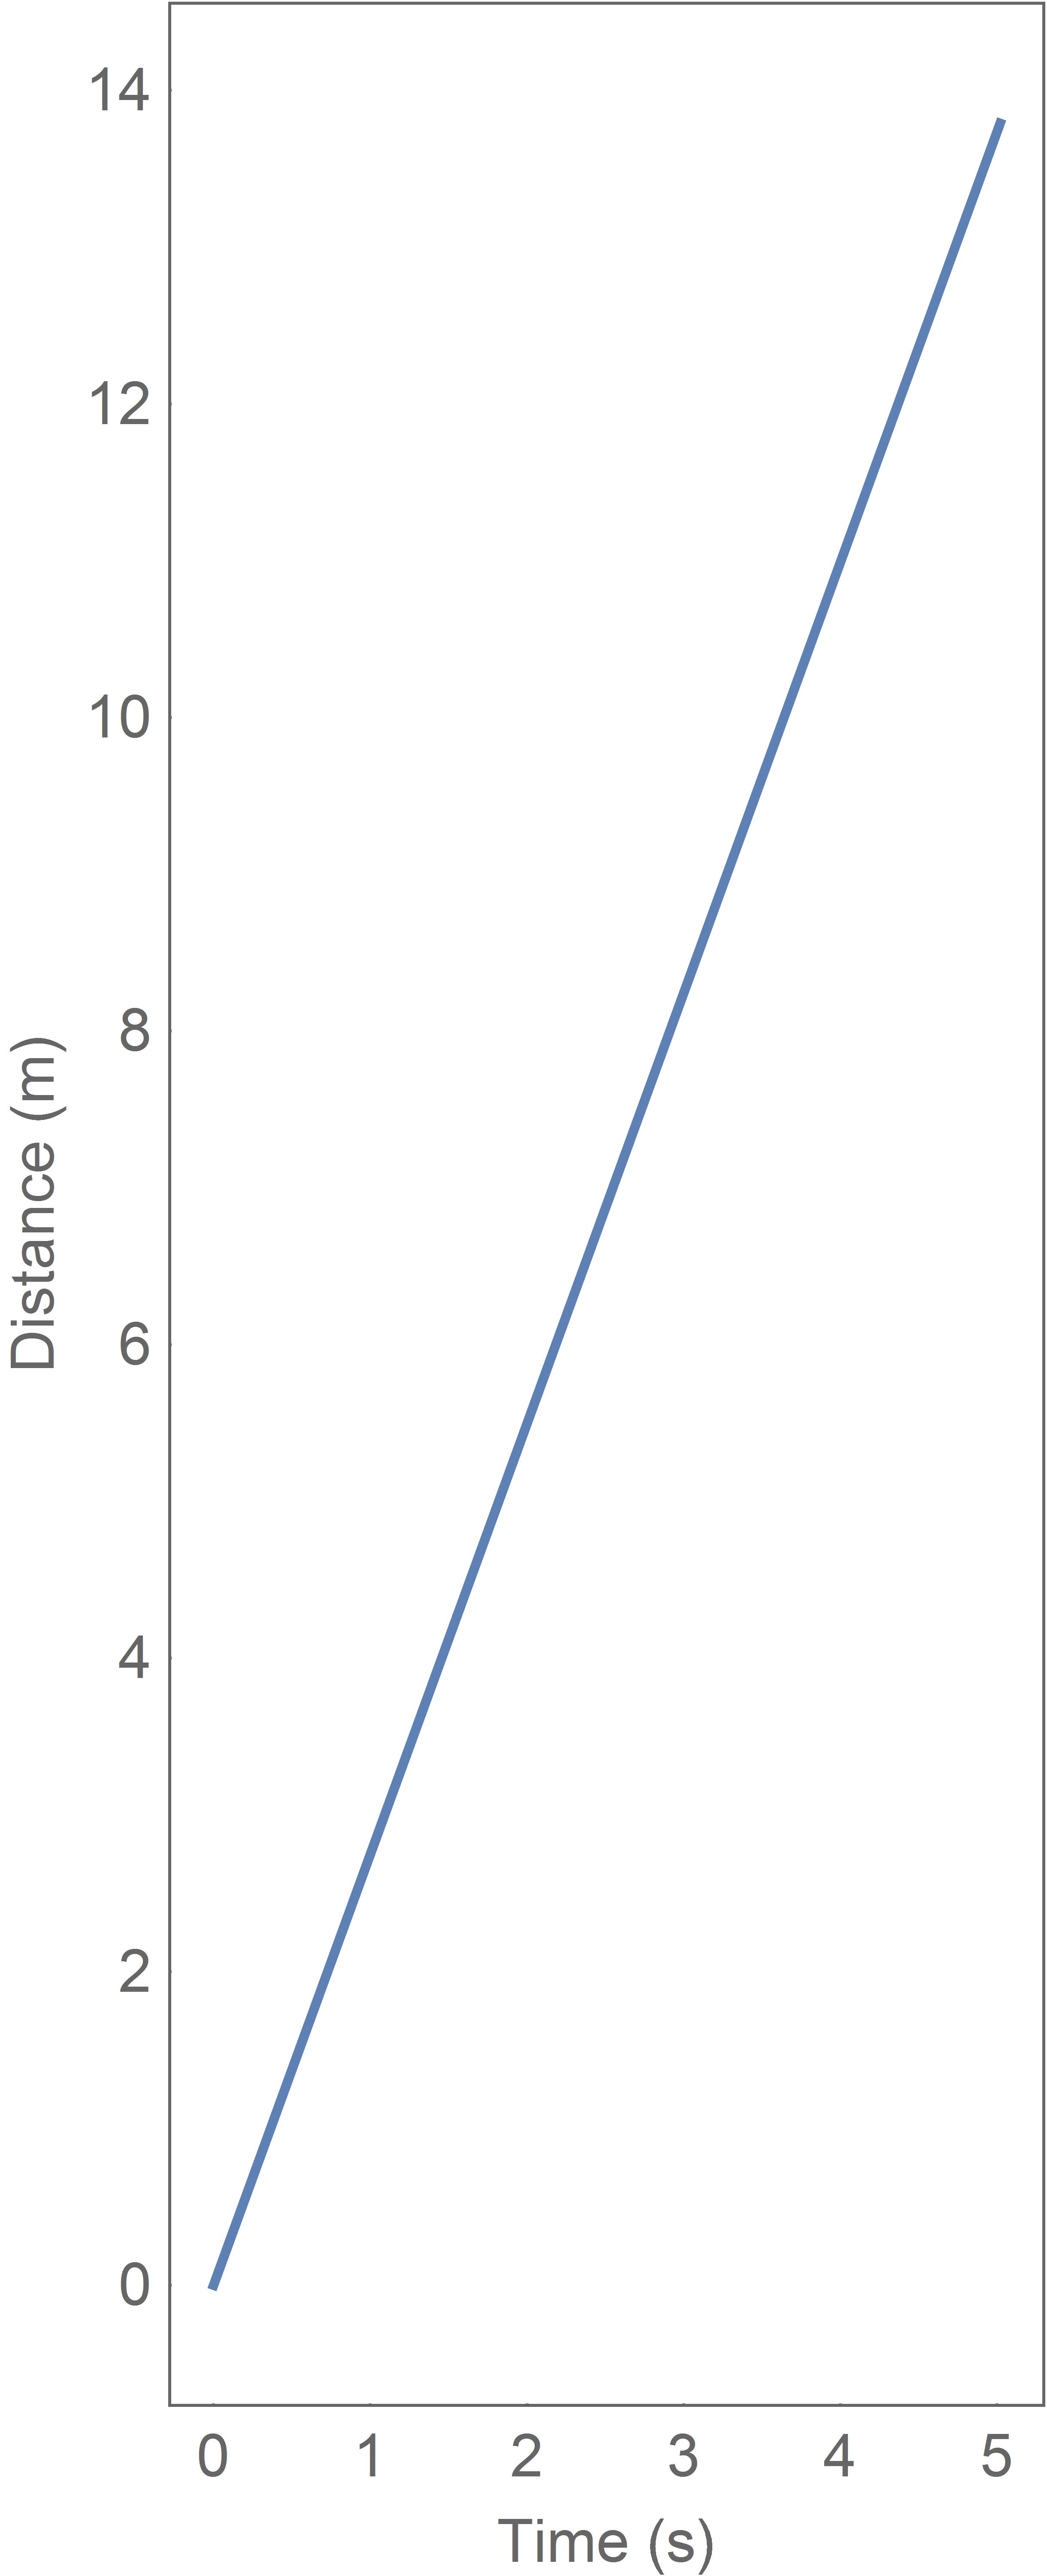
\includegraphics[width=\linewidth]{RollingWheelXY.jpg}
	\endminipage\hspace{1em}%
	\caption{The X and Y position plotted parametrically as a function of time for 5 seconds}\label{fig:RollingWheelXY}
\end{figure}

\begin{figure}[!htb]
	\centering
	\minipage{0.4\textwidth}
	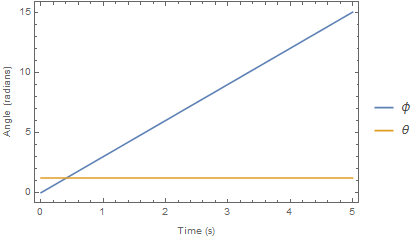
\includegraphics[width=\linewidth]{RollingWheelThetaPhi.png}
	\endminipage\hspace{1em}%
	\caption{$\theta$ and $\phi$ were plotted as a function of time for 5 seconds}\label{fig:RollingWheelThetaPhi}
\end{figure}

Based on the output in Figures \ref{fig:RollingWheelXY} and \ref{fig:RollingWheelThetaPhi}, the rolling wheel behaves as expected. 


\subsubsection{Model Implementation}

While all three approaches worked perfectly on the rolling wheel, they did not scale as desired to the much larger RipStik system.
The complexity of the system led to computations that exceeded the computer's abilities for the symbolic matrix inversion and system of linear equations.
Ultimately, numeric integration was selected to produce output.

\subsubsection{Numeric Integration}

Numeric Integration allows for the approximate computation of an integral using numerical methods \cite{WolframNumeric}.
When applying numeric integration to a differential system, stiffness is often a by-product.
The concept of stiffness is not well understood, but can generally be attributed to quick changing dynamics in a system \cite{StiffSystem}.
\par
To help develop some intuition on how stiff systems work, an example can be seen in Figure \ref{fig:stiffsystem}.

\begin{figure}[!htb]
	\centering
	\minipage{0.7\textwidth}
	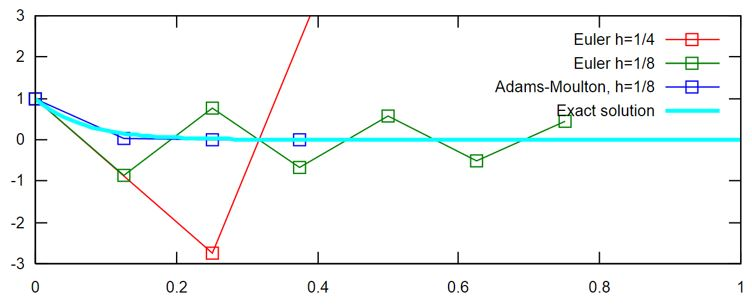
\includegraphics[width=\linewidth]{stiffsystem.JPG}
	\caption{Using numeric integration methods to approximate the exact solution to a differential equation}\label{fig:stiffsystem}
	\endminipage
\end{figure}
Figure \ref{fig:stiffsystem} shows the exact output from a simple differential equation in light blue. 
When numeric integration is attempted using Euler's method and a step size of 1/4, the approximation oscillates and completely overshoots the exact method as seen in red. 
When a step size of 1/8 is selected, there are still oscillations, but they are in a reasonable range around the exact solution as seen in green. 
When adams-Moulton method is used with a step size of 1/8, the oscillations are essesntially negligible and the approximation is almost equal to the exact solution.


\par
When a system has quickly changing dynamics, numeric integration will require increasingly small step sizes to approximate a solution without instability \cite{StiffSystem}. 
This adds computational complexity that ofteen exceeds modern technological capabilities. 
To try and reduce this computational complexity, four different numerical methods were selected to evaluate stiff DAE systems.

The QR Decomposition method decomposes the Jacobian of the derivative, breaking down the core system into two smaller systems at each iteration point \cite{Methods}.
This is represented by the following equation:

\begin{equation}
\label{eq:QR}
A = QR
\end{equation}

In Equation \ref{eq:QR}, A is any real square matrix, Q is an orthogonal matrix, and R is an upper triangular matrix \cite{Methods}.

The Collocation method linearizes the implicit DAE to m points in time, generating a system of linear equations which can be solved iteratively using Newton's Method \cite{Methods}.
The Implicit Differential-Algebraic Method uses Backward Differential Formulas (BDF) to implicity solve the DAE for derivatives to use an ODE solver \cite{Methods}. 
The BDF approximates the derivative of the function using information from previous time steps \cite{Methods}.
The BLT Method puts the system into block lower triangular form and solves subsets of the system iteratively \cite{Methods}.

While numeric integration produced results for the RipStik model, it brought its own set of challenges in the form of system stiffness.
For the RipStik, the frictionless linkages cause quick changes in the exact solution that is being approximated. 
When Mathematica attempts to numerically approximate this, it selects increasingly small step sizes to replicate these quick motions without oscillation. 
However, these increasingly small step sizes slow down the computation until Mathematica eventually abandons the attempt at numerically integrating over the chosen time interval.

\paragraph{Evaluation}\mbox{}\\
As previously discussed, four methods for numerically integrating stiff DAE systems were analyzed. 
QR decomposition, Collocation, IDA, and BLT methods were evaluated based on three criteria:
\begin{itemize}
\item The computation time was evaluated based on how long it would take for output to be generated (in seconds)
\item The duration of output was evaluated based on the length of the output computed (in seconds)
\item The reconfigurability of each method was evaluated qualitatively based on the number of tunable parameters that could be used to generate a greater length of output
\end{itemize}
A comparison of the results can be seen in Table \ref{table:evaluation}.

\begin{table}[ht]
	\caption{Numeric Integration Method Evaluation}
	\centering
	\def\arraystretch{1.3}
	\begin{tabular}{|c| c| c| c| c|}
		\hline\hline
		& QR Decomposition & \begin{tabular}{@{}c@{}}Collocation \\ Method\end{tabular} & IDA Method & BLT Method \\ 
		\hline
		Computation Time (s) & 1.2 & 26.4 & 1.2 & 1.2\\
		\hline
		Output Duration (s) & 0.6 & 5.8 & 0.6 & 0.6\\
		\hline
		Reconfigurability & Poor & Excellent & Good & Poor\\ [0.1ex]
		\hline
	\end{tabular}
	\label{table:evaluation}
\end{table}
From the results in table \ref{table:evaluation}, it is clear that there is a definitive tradeoff between computation time and length of output.
The Collocation method was able to produce output 9.7 times longer than all other methods, at a cost of 22 times longer computation.  
The gain in length of output was weighted far greater than the length of computation time, since the lengthened computation time was still feasible.

\subsubsection{Validation}

Using the Collocation integration method, 5.8 seconds of output for the falling RipStik was plotted for each degree of freedom in the system. 
As the RipStik fell, it eventually exceeded the range of validity for the Euler angles. 
This led to the RipStiks motion behaving eratically. 
As a result, only the first 1.4 seconds of the falling RipStik was plotted.

\begin{figure}[!htb]
	\centering
	\minipage{0.4\textwidth}
	\includegraphics[width=\linewidth]{fallz}
	\endminipage\hspace{1em}%
	\caption{The Z-position of the Ripstik as it falls}\label{fig:fallglobal}
\end{figure}

\begin{figure}[!htb]
	\centering
	\minipage{0.4\textwidth}
	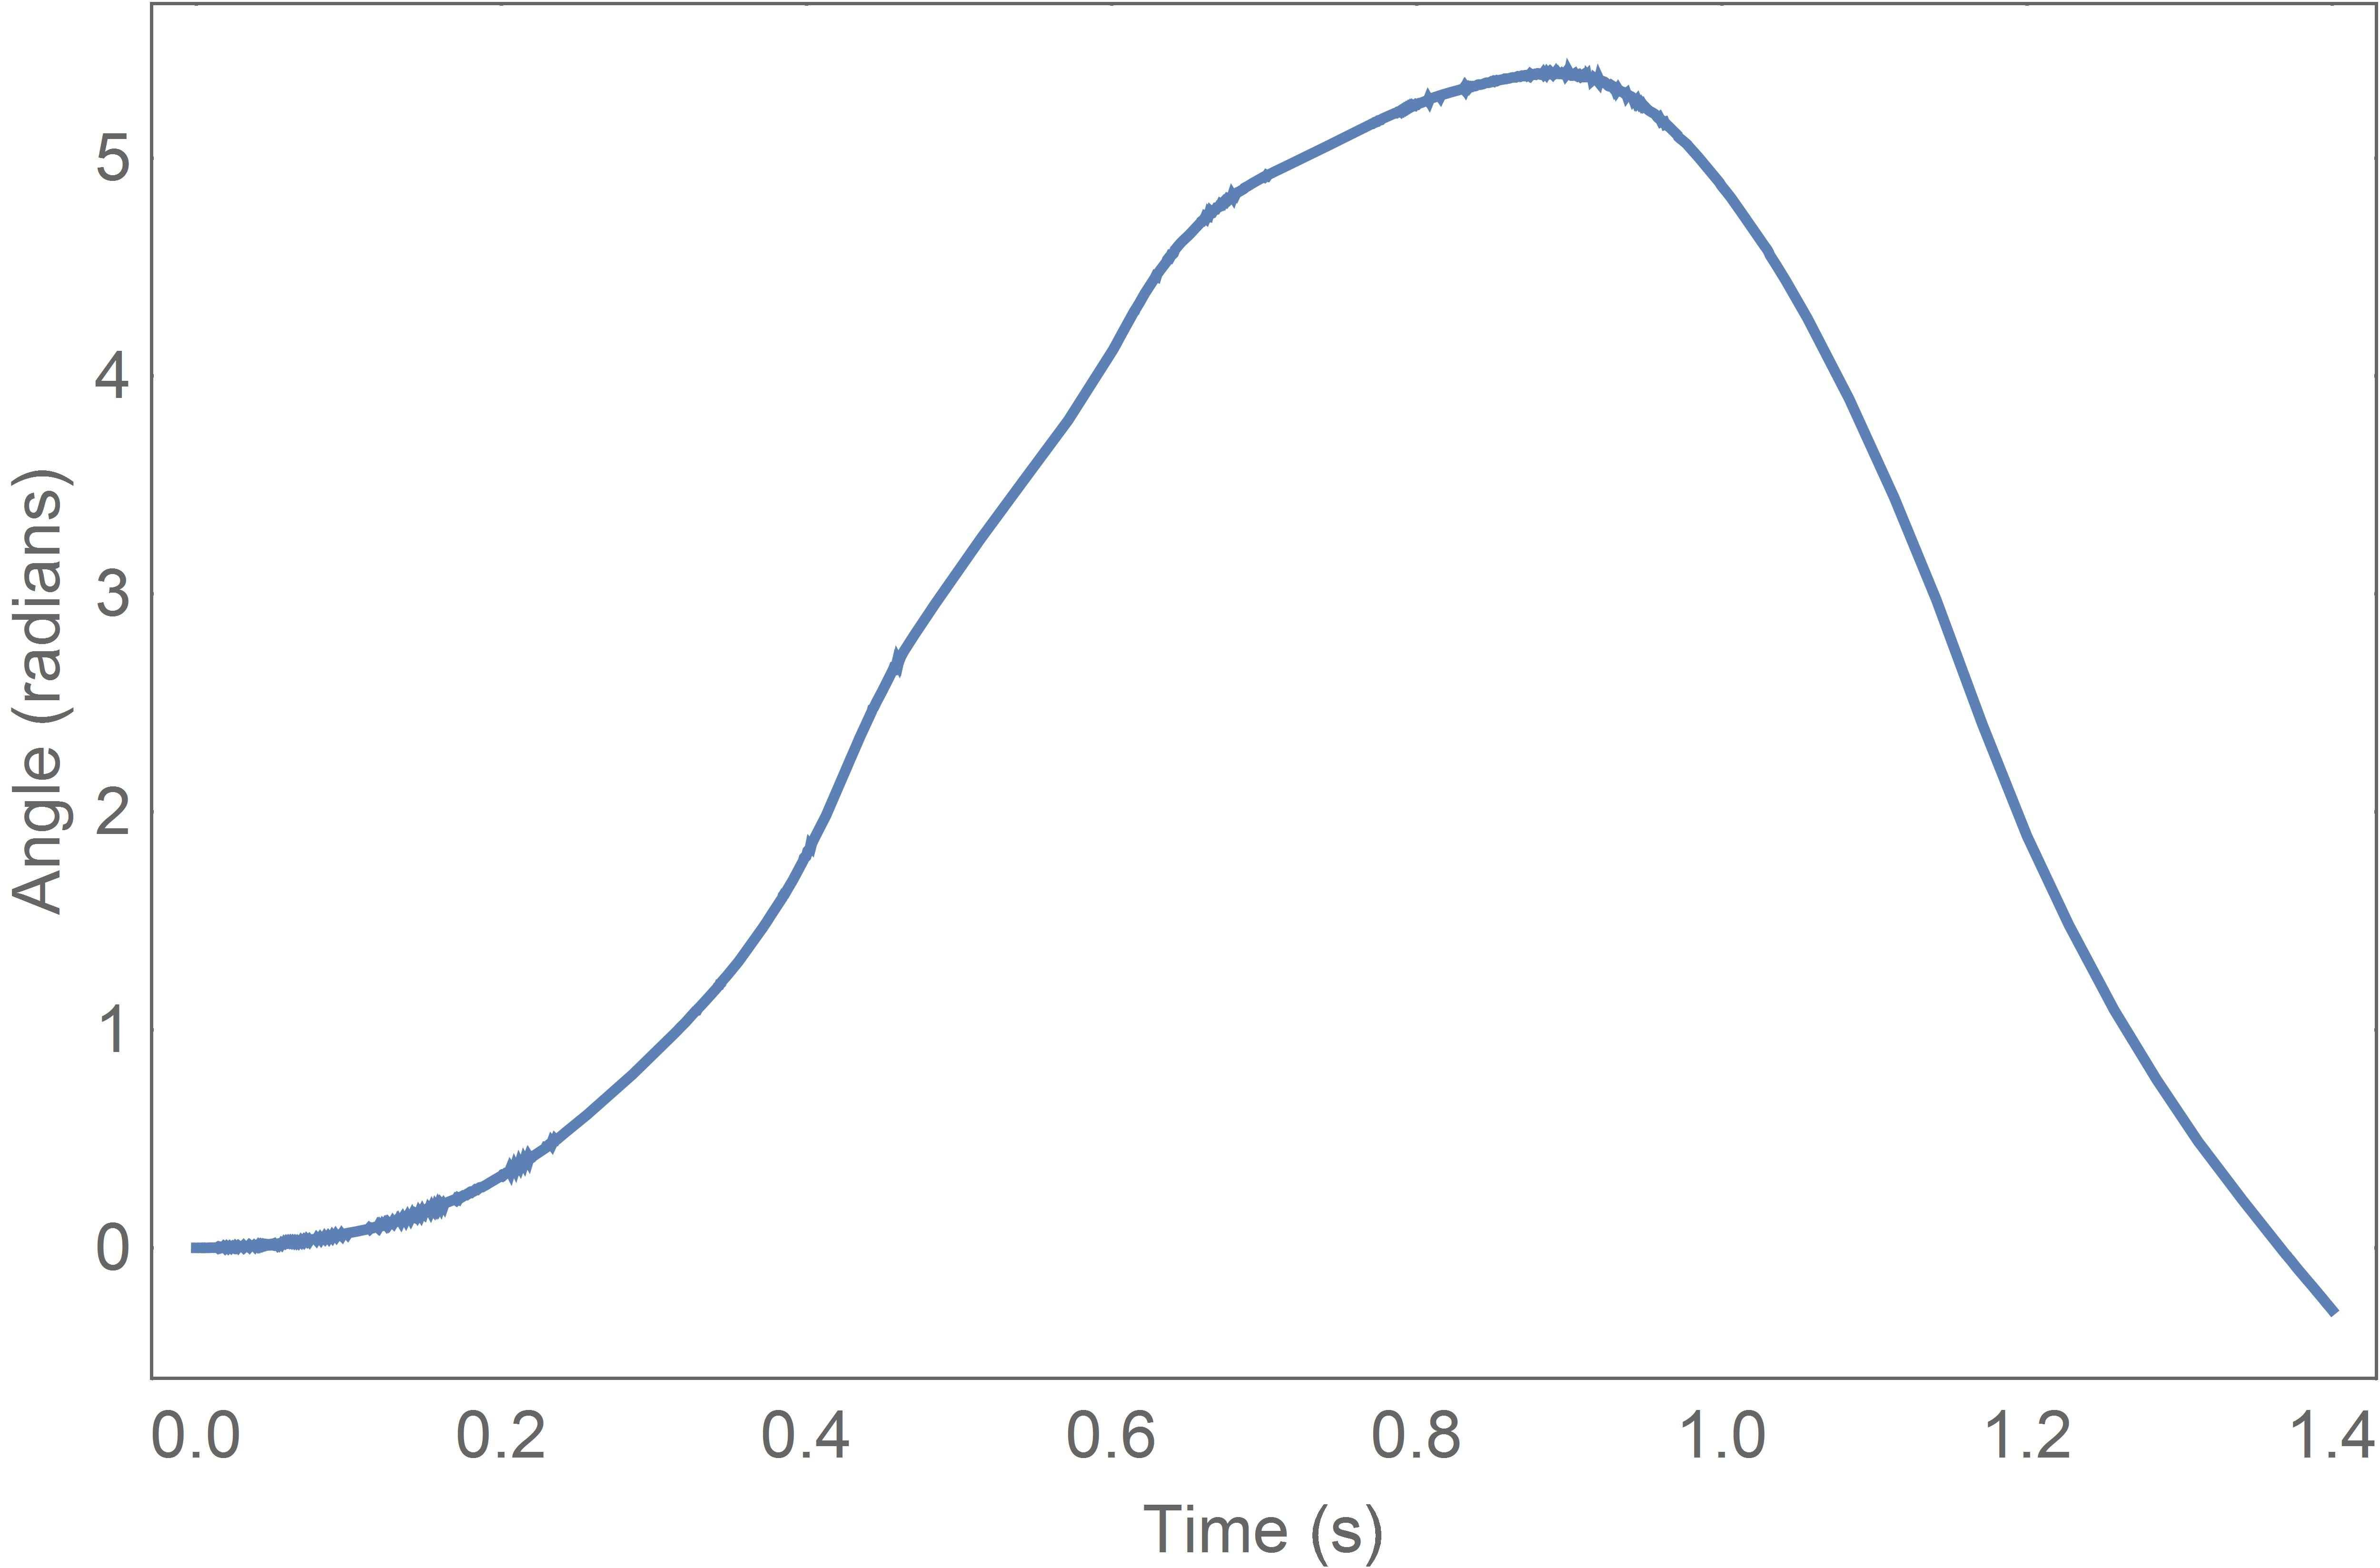
\includegraphics[width=\linewidth]{fallalphafp}
	\endminipage\hspace{1em}%
	\minipage{0.4\textwidth}
	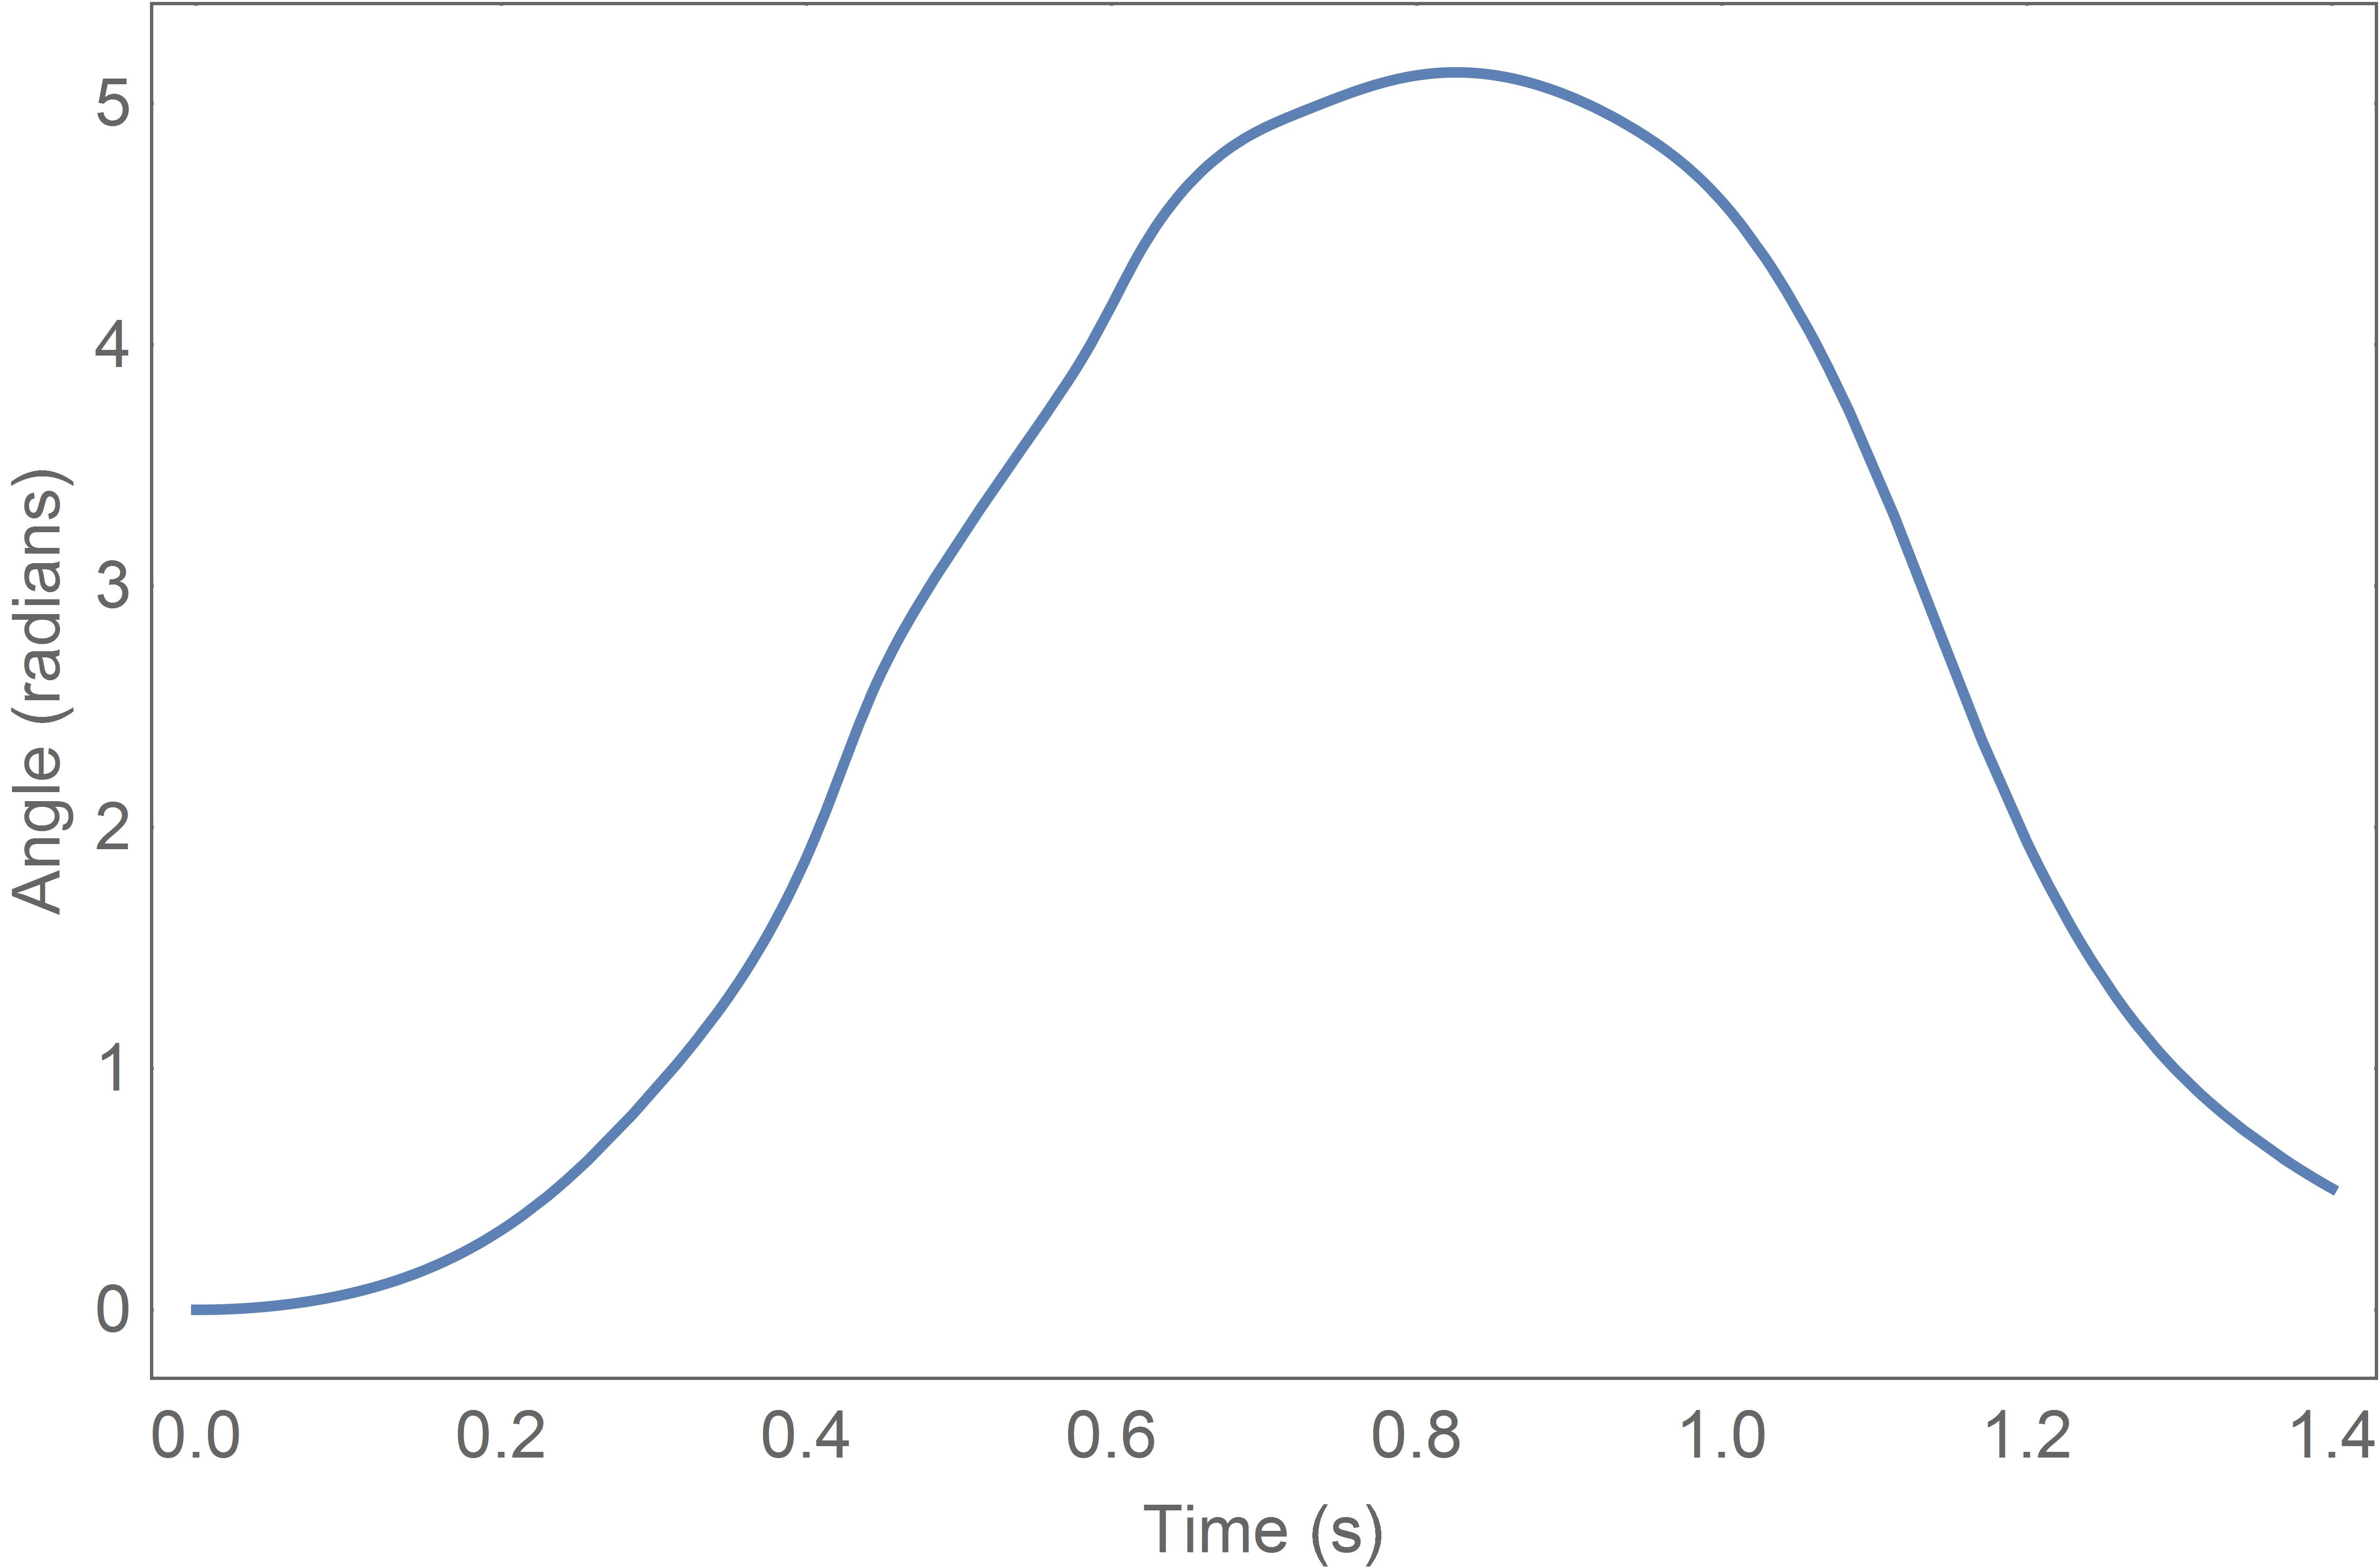
\includegraphics[width=\linewidth]{fallalphabp}
	\endminipage
	\caption{Roll of front plate ($\alpha_{fp}$) and back plate ($\alpha_{bp}$) as the RipStik falls}\label{fig:fallplates}
\end{figure}

\begin{figure}[!htb]
	\centering
	\minipage{0.4\textwidth}
	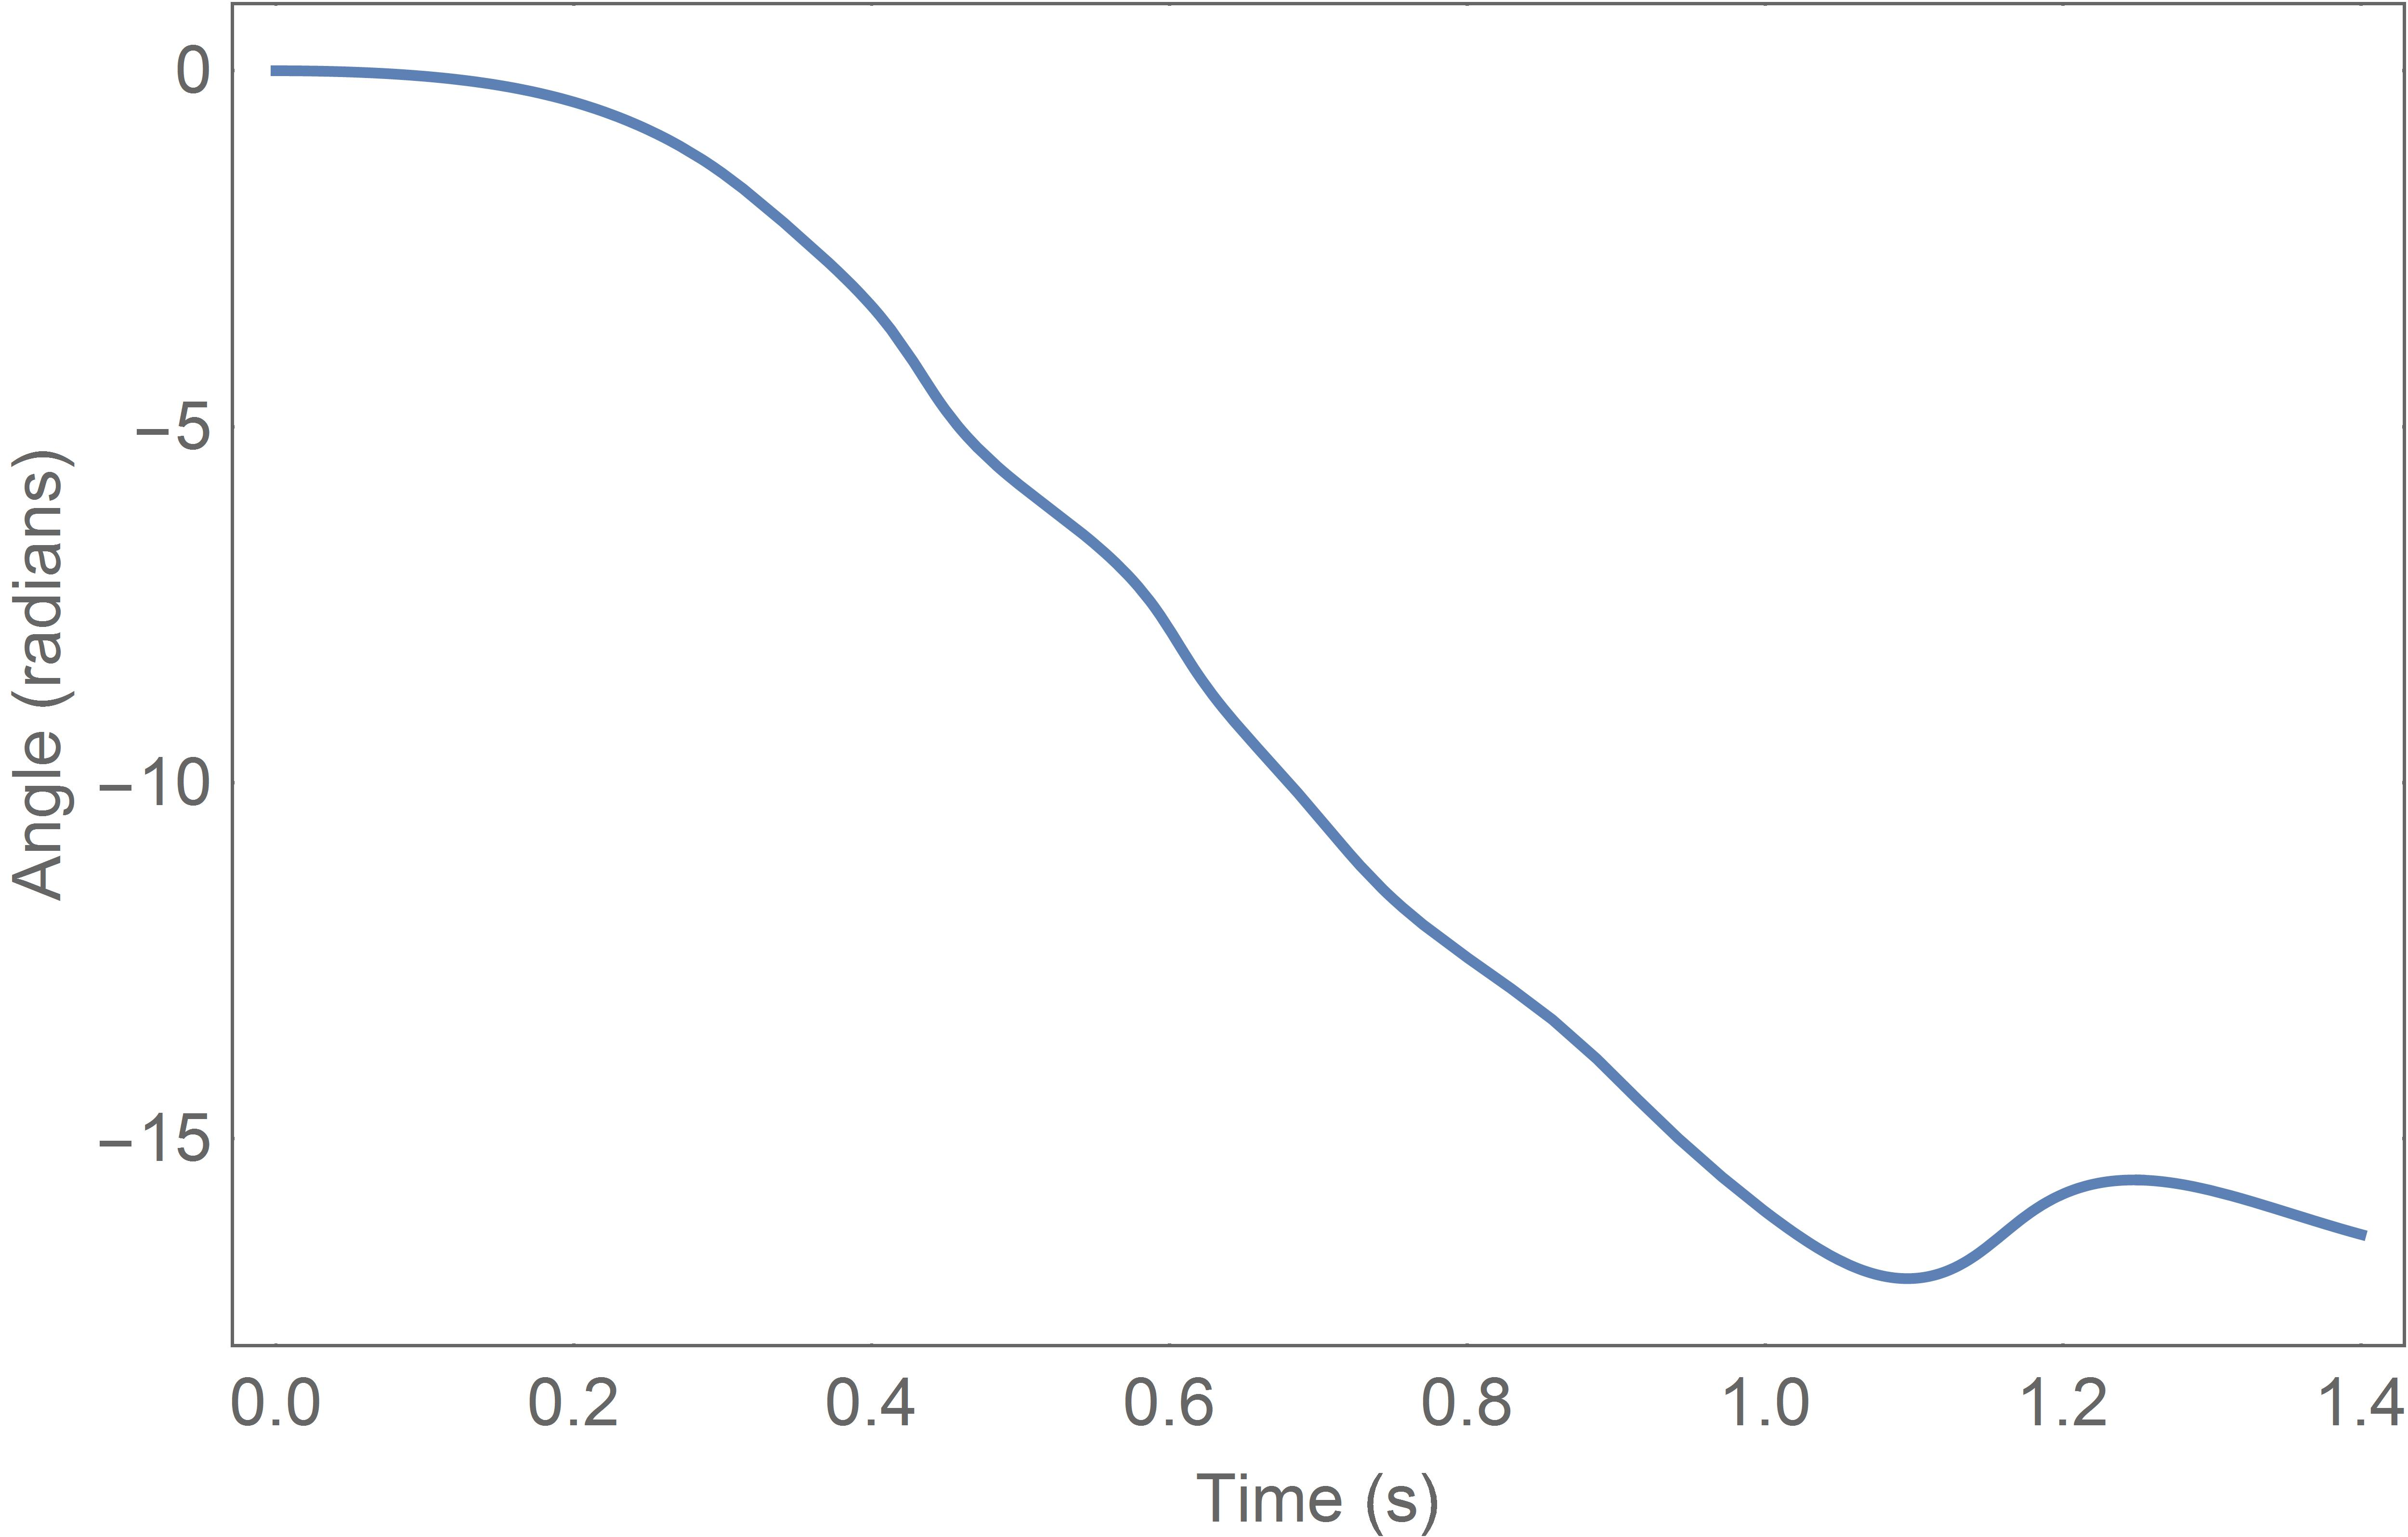
\includegraphics[width=\linewidth]{fallthetafc}
	\endminipage\hspace{1em}%
	\minipage{0.4\textwidth}
	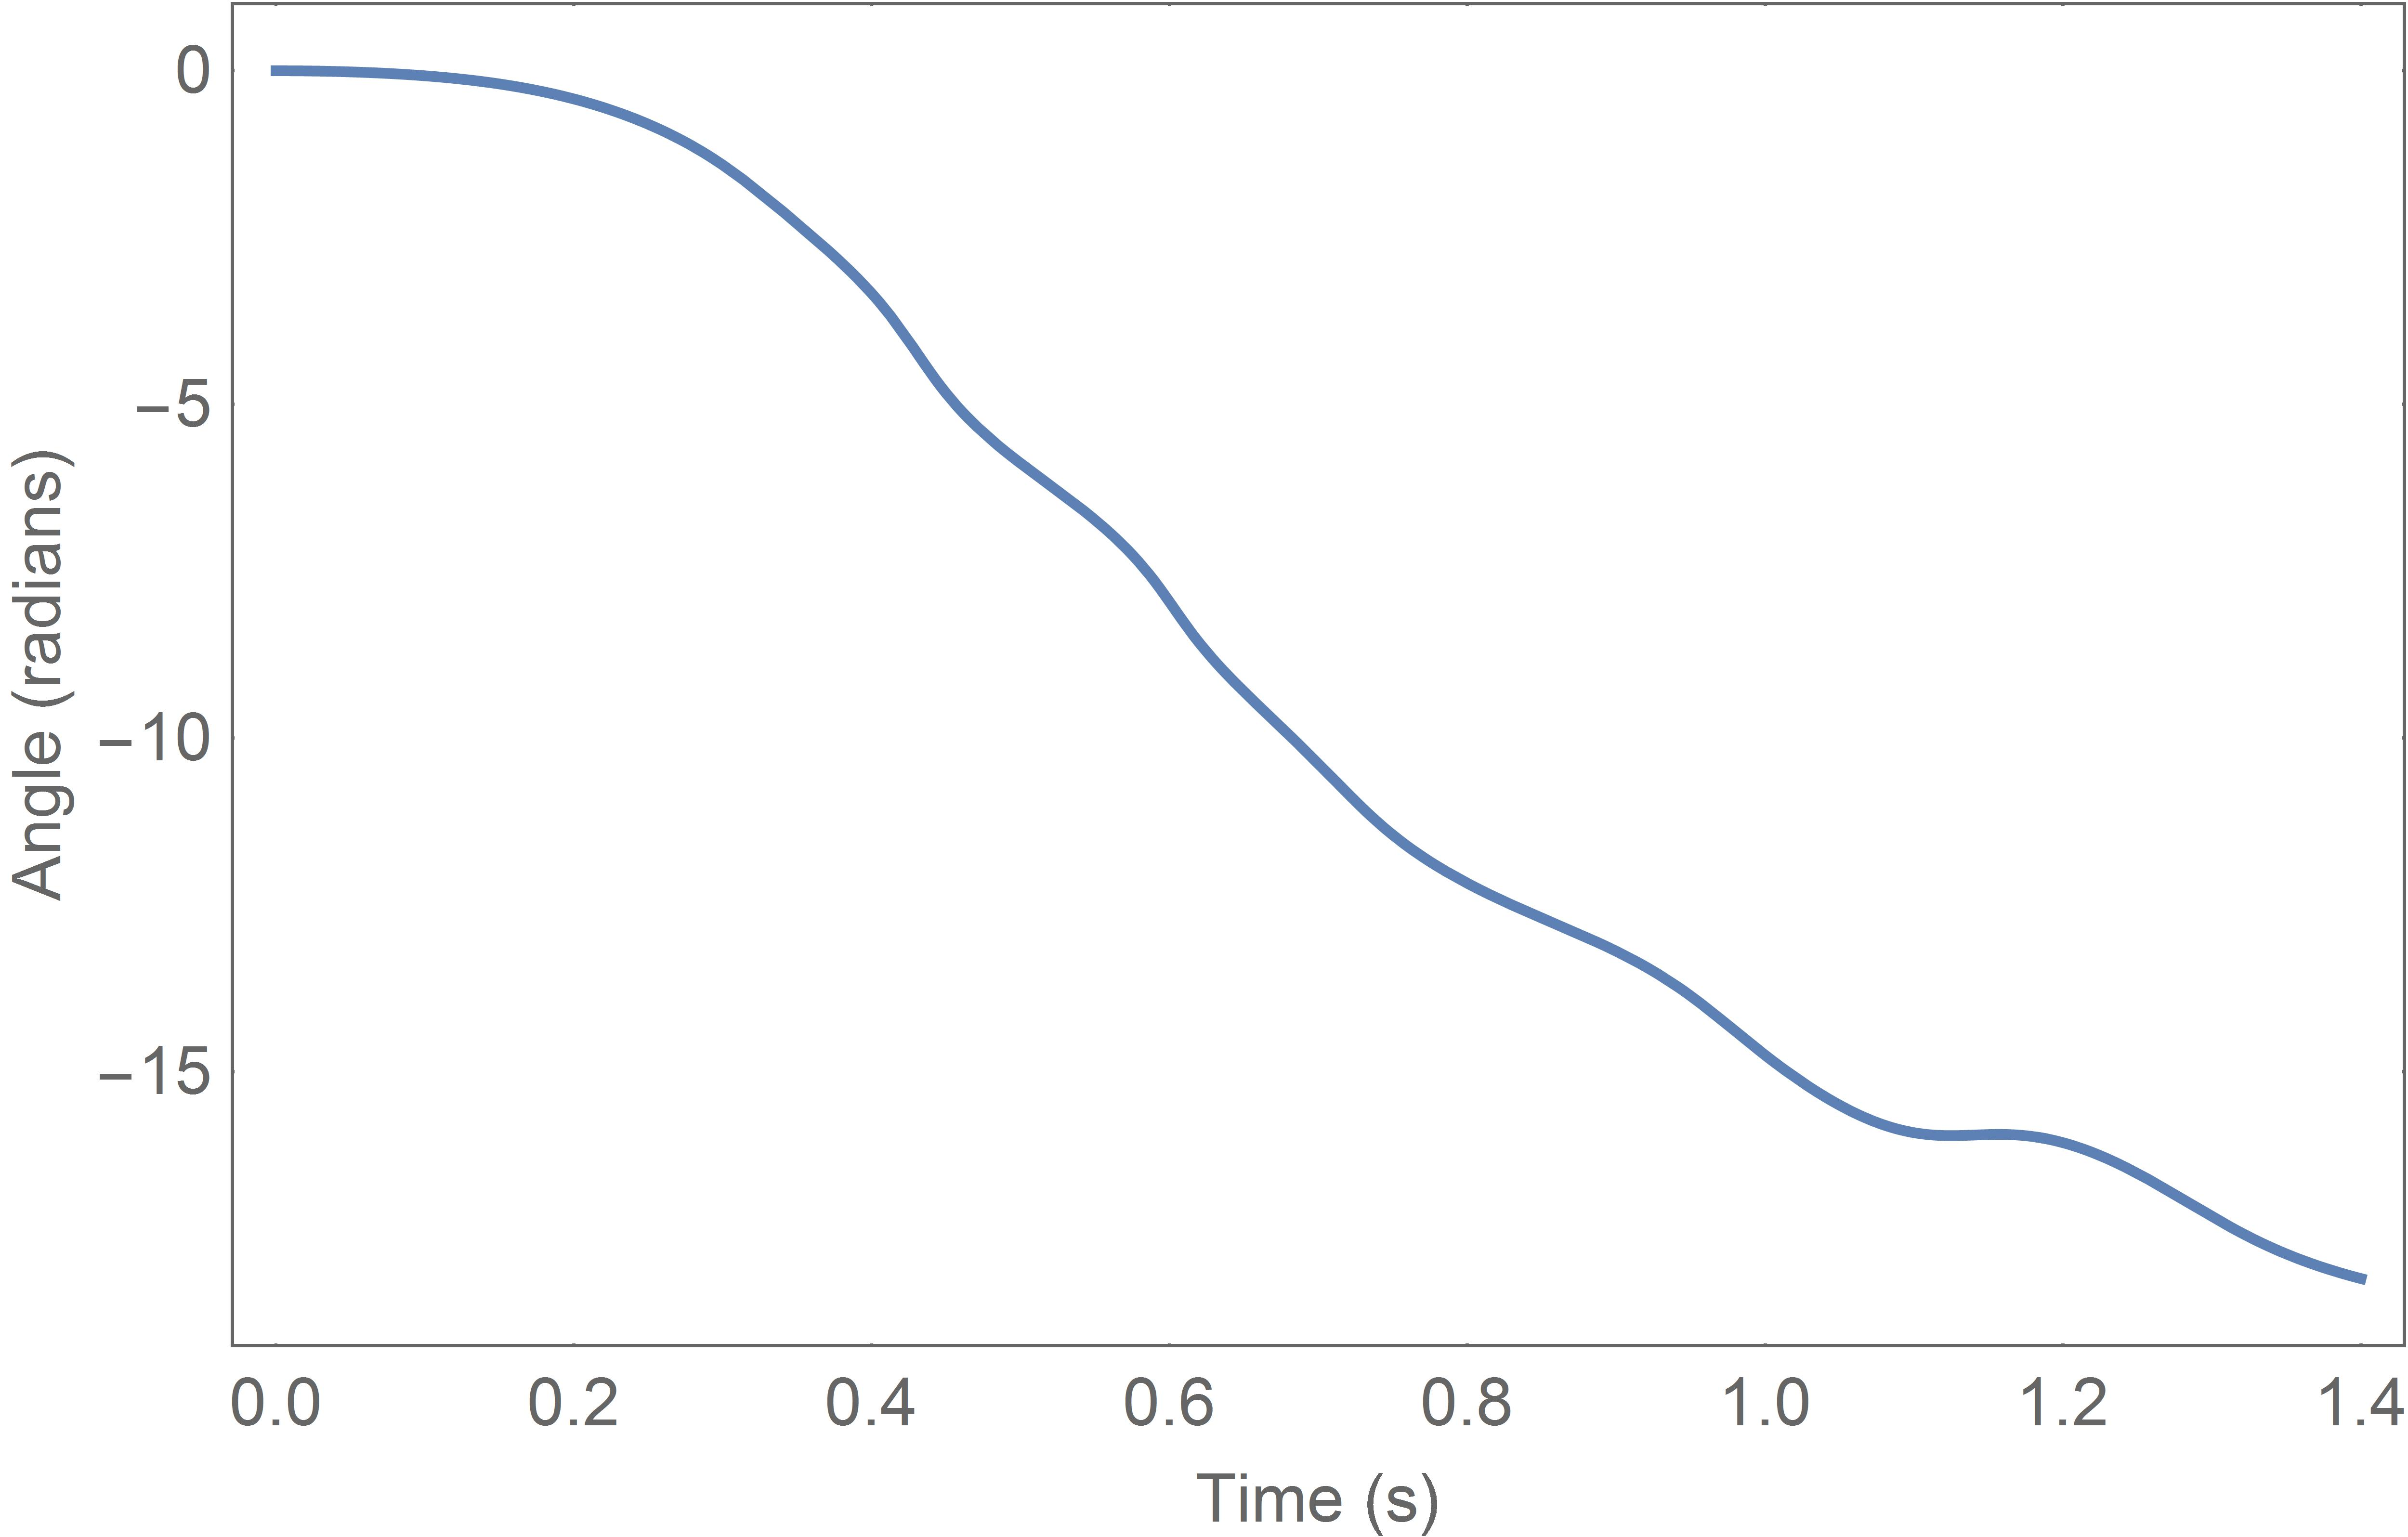
\includegraphics[width=\linewidth]{fallthetabc}
	\endminipage
	\caption{Roll of front caster ($\theta_{fc}$) and back caster ($\theta_{bc}$) as the RipStik falls}\label{fig:fallcaster}	
\end{figure}

The Z-position plot in Figure \ref{fig:fallglobal} shows the Ripstik falling through the ground plane and reorienting itself in the upright position. 
This is clearly illustrated by the oscillations shown in the first plot.


The roll of the front plate ($\alpha_{fp}$) and back plate ($\alpha_{bp}$) plots in Figure \ref{fig:fallplates} show the plates rotating almost 360 degrees, and then rotating fully back to 0. 
This clearly describes the behaviour as the Ripstik essentially flips through the ground plane.
The yaw of the front caster ($\theta_{fc}$) and back caster ($\theta_{bc}$) plots in figure \ref{fig:fallcaster} describe the motion of the casters as the RipStik falls.
The casters pivot to follow the falling motion of the RipStik and satisfy the nonholonomic constraints.
\par
An accurate visualization was produced to model the motion of the RipStik. The initial upright and final fallen over position of the RipStik can be seen in figure

\begin{figure}[!htb]
	\centering
	\minipage{0.4\textwidth}
	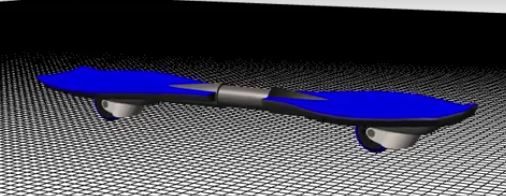
\includegraphics[width=\linewidth]{rest}
	\endminipage\hspace{1em}%
	\minipage{0.37\textwidth}
	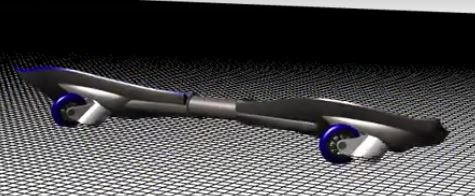
\includegraphics[width=\linewidth]{fall}
	\endminipage
	\caption{Initial upright and final fallen over positions of the RipStik}\label{fig:fallcaster}	
\end{figure}

\subsection{Linear Quadratic Regulator Control}
On the RipStik system, LQR control is intended to be used to stabilize the RipStik about the unstable equilibrium point at the upright position. 
This means keeping the RipStik platforms stable and level, with the control system forces designed to return the RipStik to this configuration under the effect of external perturbations (i.e. rider instability).

The first concern when implementing LQR control was the effect of the nonholonomic constraints on the linearization process. 
In attempting to solve for the Lagrange multipiers in the linearized equations of motion, two potential methods are considered:
\begin{itemize}
	\item Linearize the system with the unknown constraints to produce a linear DAE then solve for the Lagrange Multipliers
	\item Solve for the Lagrange multipiers then linearize the result
\end{itemize}
In his masters thesis \textit{Linearization and Stability of Nonholonomic Mechanical Systems} \cite{LinNonHolo}, S.D Yang demonstrated a sufficient condition for the commutation of linearizing the equations of motion and solving for Lagrange multipliers. 
In particular, these operations commute at critical points of the potential function\cite{LinNonHolo}.
The test case developed for LQR control consisted of a rolling wheel (as shown in section \ref{sec:testcaserw}) with an inverted pendulum attached (similar to what was shown in \ref{sec:testcaseip}). 
Since both components of the mechanical system have been previously developed and validated, minimal additional work is needed to develop the combined system. 
The system and associated dimensions are shown in \textbf{FIGURE FIGURE}.
The next steps require validating the result discussed from the thesis.

\subsubsection{Test Case - Rolling Wheel with Inverted Pendulum}

\textbf{INSERT FIGURE WITH ANGLES AND JUNK HERE}

Since it was developed in 2 dimensions, the system has 3 degrees of freedom; the horizontal position $x$, the roll angle $\phi$, and the pendulum angle $\psi$. 
Additionally, the following constants are defined: $m$, the mass of the wheel, $m_p$, the mass of the pendulum, $g$, the acceleration due to gravity, $\rho$, the radius of the wheel, and $L$, the length of the pendulum. 
Note that the pendulum is again modeled as a thin uniform rod.
The moment of inertia of the wheel is defined to be
\begin{equation}
I_w =
	\begin{pmatrix}
		J_{spin} & 0 & 0 \\
		0 & J_{spin} & 0 \\
		0 & 0 & J_{roll}
	\end{pmatrix},
\end{equation}
for consistency with section \ref{sec:testcaserw}. The rod then has a moment of inertia of \textbf{DO WE NEED A SOURCE ON THIS??}
\begin{equation}
I_p =
	\begin{pmatrix}
		\frac{1}{3}L^{2}m_p & 0 & 0 \\
		0 & \frac{1}{3}L^{2}m_p & 0 \\
		0 & 0 & 0
	\end{pmatrix}.
\end{equation}
The unconstrained Lagrangian of the system is computed to be 
\begin{equation}
\underbrace{m_P \left( g L \sin (\psi (t))- 
	g \rho + 
	\frac{2}{3}L^2 \psi '(t)^2 - 
	L \psi '(t) \sin (\psi (t)) x'(t)+
	\frac{1}{2} x'(t)^2\right)}_{\text{pendulum}} +
	\underbrace{\frac{1}{2} \left(J_{spin} \phi '(t)^2 + 
	m x'(t)^2\right)}_{\text{wheel}} = 0.
\end{equation}
Applying the Euler-Lagrange equation, the unconstrained equations of motion for the system are computed to be 
\begin{equation}
L m_{P} \psi ''(t) \sin (\psi (t))+L m_{P} \psi
   '(t)^2 \cos (\psi (t))-(m+m_{P}) X''(t)=0
\end{equation}
\begin{equation}
   -J_{spin} \phi''(t)=0
\end{equation}
\begin{equation}
   \frac{1}{3} L m_{P} \left(3 g \cos (\psi (t))-4 L \psi ''(t)+3 \sin (\psi (t)) X''(t)\right)=0
\end{equation}
Additionally, system has one nonholonomic constraint, expressed as
\begin{equation}
x'(t) = \rho\theta'(t).
\end{equation}
A control input $f(t)$ was then added to the second equation of motion, thereby applying a torque to the roll angle of the wheel.

In order to experimentally validate the presented result on commutation of linearization and solving for nonholonomic constraints, both procedures were applied to the system. 
They both produced the constrained linear system
\begin{equation}
	\frac{\left(4 J_{spin}+\rho ^2 (4 m+m_{P})\right)
   \left(L m_{P} \psi ''(t)+(m+m_{P}) X''(t)\right)-\rho 
   f(t) (4 m+m_{P})}{4 J_{spin}+\rho ^2 (4
   m+m_{P})}=0
\end{equation}
\begin{equation}
	\frac{J_{spin} \left(\phi ''(t) \left(4
   J_{spin}+\rho ^2 (4 m+m_{P})\right)-4 f(t)\right)}{4
   J_{spin}+\rho ^2 (4 m+m_{P})}=0
\end{equation}
\begin{equation}
	L m_{P} \left(4 L
   \psi ''(t)+3 X''(t)\right)=0,
\end{equation}
demonstrating that the result applies as expected for this small system. 
With the system linearized, 
\subsubsection{Model Implementation Challenges}
\subsubsection{Proposed Testing Framework}



\section{Engineering Considerations}
\subsection{Legal Considerations}

\subsubsection{Regulatory Considerations}

\paragraph{Street Legality}\mbox{}\\
Many jurisdictions have laws and regulations pertaining to the operation of personal transport vehicles, both electric and human-powered. 
Toronto and Fredricton are among many Canadian cities which have laws prohibiting the use of skateboards on public streets. \textbf{CITE? 3Chantale Nicole}
With regards to motorized transport, California had a long-standing ban on motorized skateboards which was recently abolished in the passing of Assembly Bill 2054 in 2015. \cite{OCLaws} \cite{WSJLaws}
Recently, the emergence of two-wheeled, self balancing electric scooters prompted the development of new laws and regulations. 
These devices are banned from airlines in Canada and the USA and their usage is heavily restricted or banned in regions including Toronto, Vancouver, New York City, and the state of California. \cite{leetboard}
It is imperative that a personal electric transport vehicle be compliant with relevant regulations and laws in its area of operation.


\paragraph{Intellectual Property}\mbox{}\\
In order to ensure that a personal electric transport system is commercially feasible, it is imperative that all the appropriate measures to protect intellectual property be undertaken. 
As the final product will involve the incorporation of mechanical control system to a pre-existing complex mechanical vehicle, the final product will qualify as a combinatory invention. 
A combinatory invention involves combining two or more pre-existing technologies in order to develop a new technology. 
Combinatory inventions are among the most common patents; between the years 1790 and 2010, 77\% of all patents granted involved the combination of at least two pre-existing technologies. \cite{COMB} 
A patent shall not be issued, under United States patent law, if \emph{the subject matter as a whole would have been obvious at the time the invention was made to a person having ordinary skill in the art to which said subject matter pertains. 
	Patentability shall not be negatived by the manner in which the invention was made.}" \cite{NonObv} 
\\
\\
A 2007 United States Supreme Court ruling in "KSR International Co. v. Teleflex Inc." established legal precedent for "non-obviousness" in combinatory inventions. 
Teleflex Inc. sued KSR International Co. for patent infringement pertaining to a KSR product which Teleflex claimed infringed on its patent for an "Adjustable Pedal Assembly with Electronic Throttle Control."
KSR argued that Teleflex's claim was invalid as the action was obvious. 
The United States Supreme Court ruled in favour of KSR International Co.,  
ruling that Teleflex's invention was not patentable as the combination of the two adjustable pedal assembly and the electronic throttle control was indeed obvious. 
\\
\\
In developing novel methods of personal electric transport, it is imperative that the designers consider existing patent laws and cases in order to ensure that their products can be protected.

\subsection{Professional Practice Considerations and Ethics}

Professional Engineers are bound to a Code of Ethics dictating how they must behave. Section 77 of the Professional Engineers Ontario Code of Ethics states that \cite{PEO}: \emph{"it is the duty of a practitioner to the public, to the practitioner's employer, to the practitioner's clients, to other licensed engineers of the practitioner's profession, and to the practitioner to act at all times with,
\renewcommand{\labelenumi}{\roman{enumi}}
\begin{enumerate}
	\item fairness and loyalty to the practitioner's associates, employers, clients, subordinates and employees;
	\item fidelity to public needs;
	\item devotion to high ideals of personal honour and professional integrity;
	\item knowledge of developments in the area of professional engineering relevant to any services that are undertaken; and
	\item competence in the performance of any professional engineering services that are undertaken."
\end{enumerate}}
It is an engineer's obligation to the public to ensure that a personal electric transport device be safe for public use. 
It is imperative that the control system be designed to ensure safety in the device's operation, but also minimize the impact of negligent use of the device. 
All engineers involved in the design and implementation of the control system must take all proper precautions to ensure that the system satisfy these constraints. 
The engineer must act in good faith and uphold the highest degree of professional integrity. 
\subsection{Economic Analysis}
\subsubsection{Cost Breakdown}
In order to determine the economic feasibility of an electric transport device, it was compared to traditional gas and human powered transportation devices.
An analysis was conducted based on three different metrics; Initial cost, maintenance cost and fuel cost.
The electric powered devices used in the analysis were the OneWheel and Boosted board.
The Gas powered device used in the analysis was a 2017 Yamaha Zuma 50F.
The human powered device used in the analysis was a  Raleigh Furley bicycle.
\par
Initial cost looked at the upfront costs associated with purchasing each of the devices.
Maintenance cost looked at the necessary costs required for spare parts, and yearly upkeep of each device. 
Fuel costs looked at the cost required to power each of the devices.	
The economic analysis for each method was conducted over a span of five years, and the results can be seen in Table \ref{table:econ}.

\begin{table}[ht]
	\caption{Comparison of electric, gas, and human powered transportation devices over five years (all values in USD)}
	\centering
	\def\arraystretch{1.5}
	\begin{tabular}{|c| c| c| c| c|}
		\hline\hline
		\textbf{Method} & \textbf{Device}	& \textbf{Initial Cost (\$)} & \begin{tabular}{@{}c@{}} \textbf{Maintenance}\\ \textbf{Cost (\$)} \end{tabular} & \begin{tabular}{@{}c@{}} \textbf{Fuel} \\ \textbf{Cost (\$)} \end{tabular} \\ 
		\hline
		\multirow{2}{*}{Electric Powered} & OneWheel & 1,299 - 1,499 & 340 & 25 \\
		\cline{2-5}
		& Boosted Board & 1,299 - 1,499 & 359 & 25\\
		\hline
		Gas Powered & Yamaha Zuma 50F & 2,599 & 371.40 & 155\\ 
		\hline
		Human Powered & Raleigh Furley Bicycle & 980 & 969.90 & 0\\[0.1ex]	
		\hline
	\end{tabular}
	\label{table:econ}
\end{table}

The inital cost for the OneWheel was US\$1299.00 for the base model, and US\$1499.00 for the Plus model \cite{wheelcost}.	
The initial cost for the Boosted Board was US\$1299.00 for the base model, and US\$1499.00 for the plus model \cite{boardcost}.
The initial cost for the Yamaha Zuma 50F was US\$2,599.00 for the base model \cite{Yamaha}.
The initial cost for the Raleigh Furley Bicycle was US\$980.00 \cite{Raleigh}. 
The Raleigh was selected since it was ranked one of the top commuter bicycles for 2016 \cite{BikeMagazine}.
\par
The maintenance cost for the OneWheel totaled to US\$340.00, and consisted of one replacement charger (US\$125.00), and one tune up and reload pack (US\$215.00) \cite{wheelcost}.
The tune up and reload pack consisted of a 17 point inspection, motor, battery health, hardware and firmware assessment, new footpads, new bumpers, and a new tire \cite{wheelcost}.
The maintenance cost for the boosted board totaled to US\$359.00, and consisted of replacement parts for each of the key components on the board. This includes US\$105.00 for a full set of replacement wheels, US\$100.00 for a replacement remote, US\$79.00 for a replacement charger, US\$50.00 for a bearing service kit, and US\$25.00 for a motor belt service kit \cite{boardcost}.
The maintenance cost for the Yamaha Zuma 50F consisted of a maintenance kit with lube, oil filters, fuel filters,drain plugs, and a disposable funnel \cite{YamahaMaintenance}. 
This led to a cost of US\$74.28 per year, totaling to US\$371.40.
The maintenance cost for the Raleigh Furley bicycle consisted of a tune up and drivetrain clean, along with two new tires each year. 
The tune up and drivetrain clean cost US\$150.00 per year, totaling to US\$750.00 dollars \cite{bikerepair}. 
The replacement tires cost US\$44.00 per year, and totaled to US\$220.00 \cite{CanadianTire}.
\par
The fuel costs for the OneWheel and Boosted Board were treated equally, assuming that they both use the same battery type. With the specified battery, the average yearly charging cost is US\$5.00, assuming a travelling distance 2000 miles \cite{boostedkickstart}. 
This leads to a total cost of US\$25.00.
The fuel costs for the Yamaha Zuma 50F were calculated assuming the same yearly travel distance of 2000 miles.
The Yamaha has a fuel tank that can hold 1.2 Gallons of fuel, and a fuel efficiency of 132 miles per gallon \cite{Yamaha}.
The gas price was selected by assuming that the refills are occuring in New York State, leading to a price of US\$2.448 per gallon \cite{gasprice}.
With the information provided, the average fuel cost came to US\$31.00 per year, totaling to US\$155.00.
The fuel cost associated with a bicycle is zero, as it relies only on human force for operation.
\par
From a purely monetary standpoint, the electric powered transportation is the cheapest option.

\subsubsection{Usage Characteristics}
A few other factors need to be considered, such as the range of the device, top speed of the device, and environmental impact of using the device.
The range of the device will consider total distance until the fuel source runs out.
The top speed of the device will consider the maximum speed that the device can achieve in kilometers per hour.
The environmental impact of using the device will consider the emissions generated during vehicle operation.
The three factors were measured for each device and compiled in Table \ref{table:usage}.

\begin{table}[ht]
	\caption{Comparison of the range, top speed, and emissions for the transportation devices}
	\centering
	\def\arraystretch{1.3}
	\begin{tabular}{|c| c| c| c| c|}
		\hline\hline
		\textbf{Method} & \textbf{Device}	& \begin{tabular}{@{}c@{}} \textbf{Maximum} \\ \textbf{Range (km)} \end{tabular} & \begin{tabular}{@{}c@{}} \textbf{Top Speed}\\ \textbf{(km/h)}\end{tabular} & \textbf{Emissions}  \\ 
		\hline
		\multirow{2}{*}{Electric Powered} & OneWheel & 10-11 & 15-24 & 0 \\
		\cline{2-5}
		& Boosted Board & 10-19 & 35 & 0\\
		\hline
		Gas Powered & Yamaha Zuma 50F & 253 & 68 & \begin{tabular}{@{}c@{}} 1.0 g/km HC\\ 12 g/km $CO_{2}$\end{tabular}\\ 
		\hline
		Human Powered & Raleigh Furley Bicycle & 16 & 18-19 & 0\\[0.1ex]	
		\hline
	\end{tabular}
\label{table:usage}
\end{table}

The maximum range for the OneWheel is 10-11 km \cite{wheelcost}.
The maximum range for the Boosted Board is 10 km for the standard package, and 19 km for the plus package \cite{boardcost}.
Given a fuel efficiency of 132 miles per gallon and a tank size of 1.2 gallons, the maximum range of the Yamaha Zuma 50F is 253 kilometers.
The average bicycle commuter travels a distance of 16 kilometers to and from their destination \cite{BikePaper}, but this distance can vary based on the distance the rider needs to travel and their physical fitness level.
\par
The top speed of the OneWheel is between 15-24 kilometers per hour \cite{wheelcost}.
The top speed of the Boosted Board is 45 kilometers per hour \cite{boardcost}.
The top speed of the Yamaha Zuma 50F is 68 kilometers per hour \cite{Yamaha}.
The top speed of the Raleigh Furley Bicycle is dependant on the rider, but typical speed for bicycle riders are in the range of 18-19 kilometers per hour \cite{bikespeed}.
\par
The only device that generates any environmental waste is the Yamaha Zuma 50F. The average gas scooter emits approximately 1.0 gram/km of hydrocarbons and 12 grams/km of carbon dioxide \cite{emissions}.
\par
The key trade-off to consider when selecting a device is environmental impact versus convenience.
The Yamaha Zuma 50F has a significantly higher top speed and maximum range when compared to the other devices. 
However, it generates a significant amount of emissions. The electric powered devices generate no emissions during use and are relatively fast, but can only travel short distances. 
The bicycles also generate zero emissions during use, but the top speed and maximum range are highly variable depending on the user.
As battery technology continues to progress, electric modes of transport will become an increasingly viable option.

\subsection{Social Considerations}
Two of the major social considerations that need to be addressed with regards to electric transport are rider safety and cyber security. 
These two topics are carefully reviewed below.
\subsubsection{Rider Safety}
The most recent study of skateboard related trauma occurred in 2010 and focused on the last five years of data from the National Trauma Databank in the United States, further supporting the data with comparisons to other recent studies and analysis of datasets from outside sources \cite{Injury}. The study analyzed 2270 hospital patients admitted due to skateboarding related injuries. Of these, 8\% were under 10 years of age, 58\% were between 10 and 16 years of age, and the remaining 34\% were older than 16 \cite{Injury}. One statistic the researchers highlighted was the rate of incidence of traumatic brain injury among those admitted; in aforementioned age groups, these were 24.1\%, 32.6\%, and 45.5\% respectively\cite{Injury}. While the study concluded that ``helmet utilization and designated skateboard areas significantly reduce the incidence of serious head injuries'' \cite{Injury}, this also highlights the need to develop an electric personal transport vehicle that will minimize the chance of rider injury and, if possible, reduce the severity of unavoidable falls. As the study suggests, proper protective equipment will also be crucial for any user of the proposed product. 

For the final personal electric transport system, this means preventing the automated control from applying extreme acceleration that could cause the rider to be ejected from the vehicle. Similarly, it should keep the vehicle stable in all scenarios, preventing the rider from falling off during turns or at low speeds.

\subsubsection{Cybersecurity}
With any digital system in the 21st century, cybersecurity is a key concern as it has grown far beyond simply protecting information or resources against intruders \cite{cybersecurity}. As electric skateboards have risen in popularity, they have attracted the attention of major hacking conferences. The most notable example was a recent presentation at DEF CON, ``the world's longest running and largest underground hacking conference'' \cite{DEFCONsite}, where a group demonstrated techniques for jamming and overriding the wireless control signals used by three popular electric skateboard brands, allowing them to adjust speed, apply the brakes, and permanently disable the vehicles \cite{DEFCON,wiredArticle}. This has direct implications for rider safety since a sudden stop at high speeds could cause significant injury. 

These developments must be considered for a commercial personal electric transport product since some method of wireless speed control will likely be required to allow adequate control for the rider. The DEF CON presenters noted that proprietary RF (radio frequency) protocols were particularly easy to capture and replicate using SDR (software defined radio) \cite{Radio}\cite{DEFCON} but that more modern Bluetooth features could provide sufficient security to prevent hacking using current techniques \cite{DEFCON}. Possible technologies like these will be considered to provide a solution that minimizes potential cybersecurity threats.

\subsection{Environmental Considerations}
While electric transport greatly reduces the greenhouse gases produced during operation, there is a significant environmental impact associated with the end of life cycle disassembly. The battery technologies implemented in electronic transport are analyzed below.
\subsubsection{Battery Technologies}
Modern electronic devices generally rely on rechargeable lithium-ion or lithium-polymer batteries due to their energy storage density and long product lives \cite{BatteryRecharge}. A life cycle analysis of these types of batteries revealed a high cost to the environment and to human health; high lead content (averaging 6.29 mg/L \cite{BatteryRecharge}) and cobalt content (averaging 163544 mg/kg \cite{BatteryRecharge}) both cause them to be classified as hazardous according to U.S. federal regulations \cite{BatteryRecharge}. There are risks of  resource depletion, detrimental effects to human health, and ecotoxicity associated with these battery technologies \cite{BatteryRecharge} which will have to be carefully considered when developing a solution. The potential and feasibility of next generation energy storage technologies like graphene batteries \cite{Graphene} should also be analyzed.

Batteries in personal electric transportation devices became a topic of conversation when the US government recalled over 500,000 two wheeled, self balancing scooters in 2016 due to a risk of batteries sparking, catching fire and exploding, causing at least 18 injuries \cite{CBCArticle}. This brings a clear social impact as well since there is a safety risk associated with low cost batteries manufactured in China \cite{CBCArticle}.

\section{Concessions in Design Implementation} \label{sec:Tradeoff}
There are many performance parameters of an electric personal transport vehicle that can be addressed through the design and implementation of a mechanical control system. 
These parameters include speed, handling and stability. 
However, not all parameters can be optimized through the tuning of the system; trade off in system performance is required. 
There are both trade-offs in the control algorithm and the mechanical control system.

\subsection{Control Algorithm} 
In designing a control algorithm, the primary parameters of focus are: rise time, settling time, percent overshoot and steady-state error. 
Rise time refers to the amount of time it takes for the system output to reach the desired output. 
In the context of the vehicle, a slow rise time may mean that the system is not able to stabilize a soon-to-fall rider before it is too late. 
Clearly, the rise time of the control algorithm is a priority in order for the personal electric transport device to be a viable, safe vehicle.
The settling time is also of significance to the performance of the vehicle. 
The settling time must be adequately small to ensure that the vehicle can stabilize in a practical setting. 
A lengthy settling time may result in the vehicle oscillating around a stable configuration, making it difficult to operate. 
System overshoot refers to the ability of the vehicle to return to a stable configuration in a direct manner. 
If the system overshoots the desired, stable configuration, it could result in the ejection of the operator from the vehicle. 
Clearly, system overshoot should be minimized if the control system will be used in a viable personal electric transport vehicle. 
Finally, steady-state error refers to the ability of the control system to accurately return to its stable configuration following a disturbance. 
A large steady-state error would mean that, in returning to the stable configuration following a disturbance, the system would not fully return to the original stable configuration. 
Instead, it would experience a permanent deviation from said configuration. 
The primary objective of the controller is to improve the safety and operation of the personal electric transport vehicle. 
If the vehicle is not able to accurately return to its stable configuration, it could compromise the ability of the control system to accomplish its objective.
\\
\\
Clearly, all four tuning parameters are of significant consequence in the design of a control algorithm to govern the operation of a personal electric transport vehicle. 
However, it is not possible to maximize each parameter individually in the design of a control alogrithm. 
Therefore, it is imperative that the final control algorithm be optimized to maximize performance parameters of the vehicle, while ensuring that it is robust enough to handle a variety of conditions in a variety of environments. 
Primary areas of focus in the design and tuning of the control system will vary depending on the nature of the complex mechanical system in which they are designed to govern.

\subsection{Mechanical Control System}
The control algorithm will be implemented by a mechanical control system located on the vehicle. 
This control system will require a battery power source.
As aforementioned, there are significant environmental consequences associated the manufacture and disposal of batteries. 
Minimizing the energy requirements of the mechanical control system will reduce the size and strength of battery required, thereby reducing the environmental impact of the personal electric transport vehicle.  
However, minimizing the energy requirements of the system would require minimizing the gain of the control system. 
Minimizing the gain would negatively impact the performance of the system, specifically as it pertains to the ability of the device to quickly recover from unstable configurations. 
It is imperative that the system be able to sufficiently respond to such disturbances as this is a pivotal requirement of a personal electric transport vehicle. 
Subsequently, engineers designing the control algorithm must ensure that the system is robust enough to respond to environmental changes in accordance with their duty to protect the public as specified in the Professional Engineers Ontraio Code of Ethics. 
An engineer cannot, in good faith, approve an mechanical control system design which could endanger the rider. 
Furthermore, a larger energy source will result in greater range and top speed of the vehicle. 
If the proposed personal electric vehicle is to be a viable option for urban transportation, its range and speed must be sufficiently large enough to ensure that it can reach urban destinations in a reasonable amount of time.
These are two of the outlines of an effective modern transportation system specified in the introduction. 
A trade-off between environmental considerations and project performance, constraints and ethics requires careful consideration. 
A solution in which the battery unit is sufficiently powerful enough to adequately address the performance benchmarks of the vehicle should be sought. 
\section{Future Work}

\section{Conclusions}
A comprehensive mathematical model for a RipStik is developed using Lagrangian mechanics.
This RipStik model serves as a representative example of a personal electric transport device for investigating the modeling approach and potential considerations for a stabilizing controller. 
The RipStik makes a particularly compelling example due to the unintuitive nature of the motions, large number of degrees of freedom, and limited previous work specific to the design.
Throughout the development process, a number of test cases are also presented to validate techniques before they are applied to the larger system. 
\subsection{Summary}
Modeling of the RipStik was accomplished using 5 bodies and 10 degrees of freedom.
The development begins with the establishment of the position vectors and rotation matrices for each body.
These are then used to construct the Lagrangian and, in turn, the unconstrained equations of motion for the system.
Difficulty then arises in attempting to implement nonholonomic constraints to model the behavior of the wheels.
This is due to the technical limitations associated with symbolically solving for the Lagrange multipliers in the large system of nonlinear equations. 
Numeric integration techniques are applied to overcome these limitations and produce output for the constrained model; this requires careful research and tuning due to the stiff behavior of the DAE system.
Finally, a simple model of a rolling wheel with an inverted pendulum is used to investigate the implications of nonholonomic constraints in linearization and LQR control.
\subsection{Evaluation of the Design Process}
The use of purposefully selected test cases and unit tests combined with modular, iterative code design contributed significantly to the success of the project. 
Having well defined tests outside of the RipStik provided confidence that the code would produce the desired results on the RipStik, even in cases where it was difficult to test the RipStik results directly. 
Additionally, while there was time invested implementing these test cases, it also saved time that would have been wasted evaluating incorrect code on the RipStik model (where the large scale of the system makes runtimes an order of magnitude longer). 
Constructing test cases also sometimes revealed ways to streamline the RipStik model by combining or simplifying functions that did not need to be handled separately.

Reflecting on the project, some improvements could be made to the process. 
Better metrics should have been defined for when a tool or approach must be abandoned in favor of alternates, despite that there may be associated drawbacks. 
For example, significant time and resources were allocated to attempting to solve for the nonholonomic constraints symbolically. 
This ultimately proved fruitless and the repeated attempts to evaluate the code for longer or with more computational resources were of little value to the overall project. 
Instead, a concrete timeline should have been defined (e.g. one week per approach) to continue iterating at a reasonable rate since the test cases allowed the mathematical viability of the approach to be assessed; instead, these roadblocks were often computational and somewhat secondary to the broader process.
\subsection{Lagrangian Mechanics for Modeling Mechanical Systems}


\section{Future Work}
The future of this project is a compelling challenge with the potential to produce exciting results. 
The stabilizing control results from the rolling wheel with inverted pendulum example are to be applied to the RipStik system and carefully tuned to address the engineering considerations of the project.
This will require addressing the concerns highlighted in section \ref{sec:challenge}, formally determining whether some of these concerns will arise since verifying them experimentally could be prone to uncertainty.
The RipStik model will also need to be expanded to include a rudimentary model of a rider to develop a more realistic control system that better simulates the real world riding motions.
Following successful stabilization, motion primitives will need to be developed for the motion planning problem, allowing the control system to move forward and turn to follow a path.
Some additional complexity may arise from the interaction between the stabilizing controller and the motion primitives, this will need to be carefully considered when combining the two components.
Additionally, formal testing metrics will also need to be developed to validate the completed control system and ensure it satisfies the problem definition while considering environmental, social and economic implications.

\newpage
\printbibliography

\end{document}          
